\documentclass{./template/UoYCSproject}
\usepackage{wrapfig}
\usepackage{caption}
\usepackage{subcaption}
\usepackage{booktabs}
\usepackage{tikz}
\usepackage{amsmath}
\usepackage{stmaryrd}
\usepackage{makecell}
\usetikzlibrary{positioning}

\addbibresource{main.bib}
\graphicspath{{./figures/}}
\author{Ivan Barinskiy}
\title{Bean there done what? Identifying roasted coffee bean defects using image classification algorithms}
\supervisor{Adrian Bors}
\MEng

\acknowledgements{
	I would like to thank Ben Rowe at Harmony coffee roasters and Levi and Vanessa at Vibe With coffee roasters
	for their invaluable help with sourcing and identifying the materials for the dataset and their insightful comments
	which helped inform the discussion and evaluation of the results of my project.

	I would also like to thank Adrian Bors for his advice and feedback as my project supervisor.
}

\begin{document}
	\pagenumbering{roman}
	\maketitle

	\listoffigures
	\listoftables

	\begin{summary}
		The popularity of coffee has shown steady growth over the last few years.
With the coffee industry going through several ''waves``, the latest shift in consumer focus has been towards
the clarity of flavour and the complex tasting notes that can only be extracted through careful sourcing, processing and roasting.
While green coffee production is usually a medium-to-large scale operation, coffee roasters, particularly ones targeting a
''specialty`` market tend to be very small companies, often roasting a few kilograms at a time.
Because of this, automated quality control for roasted coffee is out of reach for a significant number of coffee roasters,
for reasons including prohibitive pricing, noise, space constraints and energy consumption, requiring roasters to commit
significant manual and mental labour into manually sorting each batch.

In a collaboration with two UK-based roasters, a dataset of normal and defective roasted beans has been developed, amassing
over 2700 beans belonging to nine species and processed with six different techniques.
An image processing pipeline has been implemented using a computer vision library, digitizing and pre-processing the images.

The resulting dataset has been used to train a suite of classifiers, ranging in complexity from a KNN-based classifier to
a pre-trained state-of-the-art network, with the MobileNet V2~\cite{mobileNet} architecture displaying the best results.

The model showed potential for use in low-power or real-time systems, achieving an overall accuracy score of 95\% over 6 total classes with
1.90\% of normal beans falsely classified as defective and 2.03\% of defective beans classified as normal, making the model
a powerful tool that can assist even the smallest-scale operations at a low computational cost.

Further work has been identified as the development of a hardware prototype as well as in further developing the dataset,
with a proposal of a community-driven shared knowledge base, with roasters working together to represent the variety of coffee
available on the market.

	\end{summary}

	\chapter{Introduction}
	\label{ch:introduction}
	\section{Coffee in society}
\label{sec:coffee-in-society}
In recent years, coffee has gained more and more popularity, cementing itself as one of the most widely consumed beverages.
Along with a surge in café openings, preparing coffee at home is now an activity enjoyed by more and more people, with the average consumer being more discerning and critical than ever.

The development of the coffee industry is often described as a series of ``waves''.
The first ``wave'' made coffee an everyday staple, focusing on convenience and high availability.
During the second wave, the idea of ``specialty'' coffee first entered the consumer vocabulary, with creative recipes, flavours and textures being popularised by emerging cafés and chains.
The third wave, starting around 1980 and lasting to the present day saw a significant shift in consumer values:
rather than adding additional flavours in their coffee drinks, the consumers instead started noticing the taste characteristics of the beans themselves,
with simpler, more delicately flavoured drinks being preferred.
It is also during this time that coffee processing and roasting were moved into focus,
with the average consumer being more and more likely to differentiate and prefer a certain flavour profile over others.

The popularity of brewing ``specialty'' coffee at home has also risen during this time.
A coffee enthusiast is now more likely to own a grinder and one or more brewers, preferring to purchase whole-bean,
usually single-origin coffee, with the expectation of the resulting drink matching the advertised flavour and aroma notes.

It should also be noted that the preference in roast levels have also shifted as the waves changed.
During the second wave, when additional flavours and textures were the key focus of drinks,
a darker roast was preferred, as espresso produced with a darker roasted bean will have a more mellow,
sweet taste, with little to no acidity (though, a higher chance of bitterness if the coffee / water ratios are not correct),
and a thicker, heavier body.
With this style of preparation, an equal ratio of water to ground coffee is used, yielding a smaller, more intense espresso.

In contrast, a ``third-wave'' coffee preparation style values the acidity and floral notes that can only be retained
through a very light, gentle roasting process.
For many modern coffee enthusiasts, the lightest possible roast level is the most desirable.
While an under-roasted bean will taste unpleasant to a vast majority, with grassy, vegetal notes,
a roast level above ``medium'' is thought to mask away the harder to retain flavour notes
coming from either the coffee processing method, its origin or both.
As lighter roasted coffee is less soluble and therefore more difficult to extract,
modern coffee establishments often use higher coffee to water ratios, with 1:3 or even 1:5 ratios used to brew espresso.
Drinks brewed this way sacrifice a thicker body for clarity and brightness of flavour, exposing as much of the bean's
flavour profile as possible.
With the coffee flavour placed front-and-center, it is now more important than ever for coffee producers to deliver
the best possible quality of their product.

This shift of consumer patterns has placed a lot of importance on coffee roasters and farmers,
who are now held to a higher standard than ever before.
Even a small percentage of defects, whether in the green (unroasted) coffee or in the final product,
can ruin a brewed drink.
As environmental issues and quality control at farms is often out of the roasters' control,
it is therefore extremely important that the roasters are able to detect defects on their side
with as much precision as possible.


The following section will discuss the challenges faced by coffee roasters and producers
as well as describe the ``state of the art'' of quality control in coffee production.

\section{Coffee production challenges}\label{sec:coffee-production-challenges}
The worsening climate conditions, rising consumer expectations and economic instability are just a few of the challenges
faced by the coffee roasting industry.
As many roasteries are quite small businesses, addressing supply chain issues is often beyond their control,
with roasters having to perform secondary quality control to address the shortcomings of the previous stages in the beans'
journey.

Defective green coffee beans can seriously damage the flavour of the finished product.
The most common defect occurs when the coffee cherry does not develop the necessary sugar content
due to being harvested before fully maturing or disease of the plant:
the beans within these cherries do not respond well to roasting, developing an extremely unpleasant flavour
which is typically compared to burnt paper, with an astringent, drying sensation in the mouth.
Such beans are commonly referred to as ``quakers'' and, when roasted, can be identified by
an uneven, spotty exterior as seen on figure \ref{fig:quakerBeanExample}.
The spotty pattern develops due to the lack of sugar, preventing the bean from fully caramelising during roasting.
\begin{wrapfigure}{r}{0.5\textwidth}
    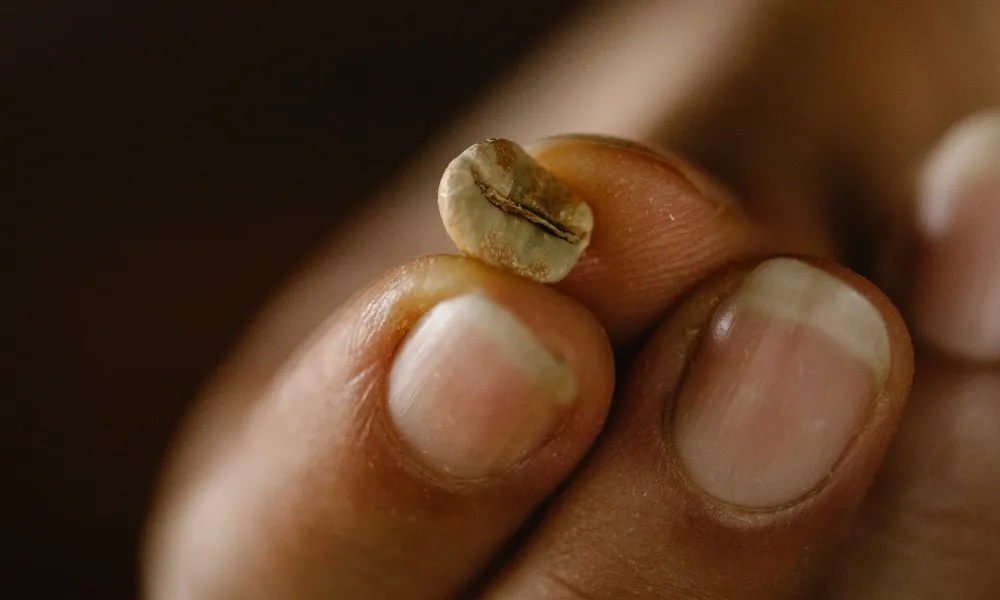
\includegraphics[width=0.5\textwidth]{quaker-coffee-bean}
    \caption*{Source: \cite{quakerBeanImg}}
    \caption{An example of a ``quaker'' coffee bean.}
    \label{fig:quakerBeanExample}
\end{wrapfigure}
The unpleasant flavour brought along by such beans is extremely potent, with just a few being able to ruin a large batch
of otherwise acceptable product.

Apart from harming the taste of the roasters' products, such beans can also prevent the roasters from achieving certain
certifications or using certain marketing language.
The Specialty Coffee Association (SCA) is one of the most influential regulatory bodies in the coffee industry.
The term ``specialty'' can only be used to describe coffee when certain criteria are achieved:
each batch of green coffee is roasted and tasted, with the tasters awarding points for various aspects of the drink's flavours.
In order to achieve specialty status, the coffee has to earn over 80 points, as well as being free from the previously mentioned defects.

As the ``specialty'' mark is often necessary for a roaster to stand out among its competition and make itself known to
coffee enthusiasts, quality control is one of the most important tasks that a coffee roaster faces on a daily basis.

\section{State of the art in coffee quality control}\label{sec:qc-state-of-the-art}
Despite the previously described importance of quality control, the automation options are surprisingly limited,
requiring many medium-to-small scale roasters to perform their quality control manually.
While the knowledge and expertise of many roasters allows them to perform this task relatively easily,
it still requires a significant amount of time and manual labour, preventing the roasters from performing other tasks.
Furthermore, this approach does not guarantee repeatable or even correct results,
depending fully on the judgement of the person performing it.

It should be noted that some commercial solutions are offered:
industrial scale colour graders can provide a high degree of accuracy and efficiency.
These machines use image recognition to place the beans in one of several pre-determined categories,
using blasts of compressed air to remove defective beans as they fall through the air.
\begin{wrapfigure}{r}{0.5\textwidth}
    \includegraphics[width=0.5\textwidth]{colour-sorter-scale}
    \caption*{Source: \cite{colourSorterImg}}
    \caption{A typical colour grader in a coffee roasting facility}
    \label{fig:colourSorterExample}
\end{wrapfigure}
These machines, however, are often a poor fit to all but the largest coffee roasters due to several reasons:
\begin{itemize}
    \item Prohibitive pricing
    \begin{itemize}
        \item Test
    \end{itemize}
    \item Large size
    \begin{itemize}
        \item Test
    \end{itemize}
    \item Unknown training dataset
    \begin{itemize}
        \item Test
    \end{itemize}
    \item Scale of production
    \begin{itemize}
        \item Test
    \end{itemize}
\end{itemize}


\section{Research aims}\label{sec:research-aims}

	\chapter{Literature review}
	\label{ch:litreview}
	When reviewing the literature for this project, the available information fell into
two categories: on one hand, it was important to consult papers describing past attempts
at classifying coffee beans, especially those that proposed methods for doing it
at scale.
On the other hand, looking at the wider world of image classification
revealed useful details and approaches to classifier architecture that informed
the decisions made in this project.
Overall, considering the history of image
classification as a field and its applications in the coffee industry built the
information background that enabled the development of the prototypes in this
project.

The overall picture gathered from reviewing the literature related to the task at hand
suggests that identifying items as small as coffee beans is definitely
possible, although not without some degree of effort invested in the process.
Several
of the reviewed papers claimed great results, though for many, the data gathering
and cleaning process involved rare or expensive equipment.
The following sections will outline some of the most frequently used image classification algorithms
and their application to coffee bean quality control.

\section{Commonly used image classification algorithms}
\label{sec:lit-review-general}
\subsection{K-nearest-neighbours classifiers}
On the conceptually simpler side of image classification algorithms lies the
KNN classifier~\cite{knnOverview}, a method of unsupervised learning, where the
classifier ''learns`` from the differences between the datapoints rather than
their labels.
A KNN classifier's main benefit is the lack of training time:
instead, the images are compared to the others as soon as they are available.
This allows for rapid prototyping and a quick implementation time at the cost of
the resources needed to make each decision when running the model.
Despite this tradeoff,
versions of the KNN architecture remain a popular choice for image
classification to this day, and, with some modification, solve the large resource
requirements by utilising advanced data structures, such as in the case of the
KD-KNN algorithm~\cite{kdtreeKNN}.

Since the algorithm requires the calculation of ''distance`` between any given
datapoints, several metrics of calculation exist, such as Euclidean, Manhatan and
more.
The choice of the distance metric as well as the value of K must be picked
experimentally, with a technique such as grid searching.
Overall, the KNN algorithm
provides a quick and efficient way of prototyping an image classifier, however
the simplicity comes at a cost of the need to manually pick the necessary
hyperparameters to get the best out of the architecture.

An application of this classification method to a coffee-related problem can be seen in a 2019 paper by Oliveri et al.~\cite{hyperspectralGreenOliveri}.
Using a KNN classifier to assign the closest category to a given bean image, the authors
aimed to classify green (unroasted) coffee beans.
Apart from the ''normal`` class, three further defects were identified, including dehydrated beans, beans extracted from
underdeveloped cherries and ''black`` beans, which were extracted from cherries that prematurely fell off the tree and died.

The images were taken in batches, using a hyperspectral scanner, which captures light
beyond the visible frequency range.
The capturing
of images was automated using a conveyor belt feeding rows of beans of the same category
under the scanner.
While the extra equipment required for this approach
introduces extra costs and may be better fit for a commercial application, the technique
of splitting an image of a row of beans into groups of individual images, all
resized to the same dimensions provided a great way to simplify and speed up the
data gathering process for this project.

The authors did not develop any physical apparatus to separate the defective beans
in their paper, however they were able to process images of groups of beans, highlighting
defective ones on the original image.
This approach fits really well with the
constraints and aims of this project, as being able to identify defects and determine
their place on the original image would already lead to a significant saving of effort
and time for the potential users.

Another strength of Oliveri et al's paper is in their iterative and transparent approach
to the development of the model.
The authors were one of the few who mentioned
cross validation as part of their project and explained the choice of the number
of neighbours for their classifier.
Furthermore, they admitted that due to the
rarity of certain bean defects, they were not able to gather enough samples to add
them to the classifier as well as having to remove a number of beans from the sample
pool to make the ratio of beans in each class as even as possible.

While the above shortcoming, coupled with a lack of reporting on the species or
processing of the beans, identifies areas for improvement, the overall approach
shows great potential in identifying defects.
The application of the model and its
design have influenced the research process for this project, which, with a more
varied dataset, aims to explore the topic of KNN classification further.

Despite KNN classifiers' popularity, they are not without their drawbacks, with the main one relating to
the difficulty of representing image data in a less high-dimensional and space-ineffective way.
To convey enough information about a given image, complex pre-processing procedures, such as PCA or texture analysis may
be needed.

\subsection{Neural networks}
A more modern and complex solution can be found in neural networks.
These classifiers
attempt to mimic the human brain, where each neuron activates or ''fires`` only
if some condition (the ''activation function``) passes a certain threshold.

Neural networks can be used for more than image classification and are an
actively developing topic to this day, however some network architectures utilizing convolution layers are known
for their performance with images and are commonly used as the baseline for more
domain specific applications.
Some classic examples of such architectures include LeNet~\cite{leNetOverview}
and AlexNet~\cite{alexNetOverview}, which are often used for datasets containing
smaller (in terms of pixel resolution) images, making them a good potential
starting point for use in this project.
AlexNet in particular has shown great potential
with image datasets, such as CIFAR-10~\cite{cifar10}, which, given that the
number of roasted coffee defects roughly matches the number of classes in the
CIFAR-10 dataset, suggests that an architecture similar to AlexNet may be a good
candidate for this project.

A notable use case of neural networks for coffee bean classification was done by Chen et al.~\cite{hyperspectralChen},
who have achieved an accuracy of 98.6\% when
classifying green coffee beans.
While the purpose of their paper is slightly different,
focusing on optimising a different stage in the coffee supply chain, their approach
to data collection and processing provided valuable insights serving as a great starting
point for the implementation of this project.
Similar to this project, the authors have identified several green coffee
defects to classify: insect damage, black beans (ones that have prematurely
fallen off the tree and could not develop) and bean fragments.

Similarly to Olivieri et. al.'s paper, image gathering was automated and involved capturing
several light spectra to extract more information from each image compared to visible light photography.

The authors, using neural networks to classify the images, have provided several
classifier architectures.
While the highest-performing network in their study (a
3D-CNN) required leveraging the hyperspectral data provided by the scanner, the
2D-CNN architecture they described used only the spatial data of the images.
Interestingly,
the CNN-based classifiers boasted fast prediction time, with the authors developing
a real-time sorting device.
While physical prototypes are beyond the scope of
this project, knowing that near real-time classification speeds are possible with
this architecture suggests that this approach could fit the task at hand well.
Furthermore, Chen et al.\ employed a dimensionality reduction algorithm (PCA)
for their model, which has improved the overall accuracy when reducing the hyperspectral
data down to 3 components.
This increase in performance could also be
investigated and leveraged in this project.

Despite the high performance and large dataset in Chen et al.'s paper, the real-world
performance of any model could be improved by a more diverse dataset, showing either
more defects, more coffee varieties, or both.
This project aims to cover this
gap by utilising beans processed by various methods, from several distinct origins
and species.

A 2017 paper by Nasution and Andayani~\cite{manyRoastLevelsNasution} shows a
departure from the previous two paper both in its approach to data gathering as
well as the overall aim.
Instead of focusing on green coffee defects, they
instead focused on coffee roast levels, aiming to classify the beans' degree of
roast on a scale of 16 levels, from completely green to burnt.
The images were
gathered using a common smartphone camera and resized to the same dimensions, with
each image containing a single bean.
For their classifier, the authors chose a backpropagation
neural network, with the images first processed by a gray level co-occurrence
matrix (GLCM), a technique that allows to develop insights into textures of surfaces
from an image.

Overall, the authors claim an accuracy of 97.5\%, however the report lacks
transparency in the total number of samples as well as the way classes were
determined, with some roast levels only having a slight difference in hue.
With
such a fine-grained scale of roast levels, it is difficult to see how the authors
were able to find a sufficient quantity of beans at each level and classify them
without samples of one class mixing into others.
Despite this lack of
transparency, the paper still provides a valuable look at how a task similar to the
one in this project can be done without requiring complex and expensive equipment.
The results achieved by the paper, while being able to benefit from more clarity
in reporting, suggest the possibility of developing a classifier that:
\begin{itemize}
	\item Is able to work on visible-light images only

	\item Is able to pick up on small changes in the surface of the beans

	\item Differentiates roasted beans, which may have less colour variation than
	green beans with a similar degree of accuracy
\end{itemize}

A paper with one of the closest aims to the project at hand was written by Shao et al.\ in
2022\cite{rgbDeepLearningShao}.
Similar to this project, the paper aims to
classify roasted beans, with the authors identifying a similar number of bean defects.
Interestingly, the authors identify ''peaberry`` beans or beans with an exceptionally
small, round shape, as a defect,
whereas many coffee consumers and producers believe that such beans provide a
flavour advantage over regular beans and market them as the more desirable
species.
It should be noted that this paper highlights the usefulness of automated
bean classification: with a sufficiently well-trained model, a physical prototype
could be implemented to sort the beans, allowing the producers to discard or
separate the bean classes they deem valuable or defective.
In that regard, Shao
et al's paper is an important showcase of the economic benefits brought along by
automation of the coffee quality control process.

The authors have also provided an automated method of data gathering, utilizing a
rotating wheel to briefly hold the beans in front of a camera.
Similar to
Nasution et al.\cite{manyRoastLevelsNasution}, the authors worked with RGB images
and did not employ any light spectra beyond the visible one.

The authors have used an existing, well-researched CNN architecture to develop
their model, with 11 total layers, achieving an accuracy as high as 96\% with the
lowest score of 88\% across the seven identified classes.
Similar to commercial solutions
described in section~\ref{sec:qc-state-of-the-art}, the authors have used an air
compressor to automatically remove defective beans, proposing a lower-cost, more
customizable solution of coffee quality control.

While the authors did not make any mention of the number of beans of each
category they gathered or the breakdown of origins and processing methods of the
beans, the high total number (1700) of the beans suggest that there was sufficient
data to train the model.
A potential improvement could be seen in a more varied
dataset with a more even breakdown of classes.

Apart from the described usage of expensive and complex machinery to
automatically gather the images and remove the defective beans, the approach taken
by Shao et al.\cite{rgbDeepLearningShao} showcases a low-cost approach, requiring only a visible-light camera
and sufficiently powerful hardware to train the model.

While gathering data for a prototype project is a relatively straightforward task,
a real-life coffee roaster may have access to a much greater number of defects
and may be in search of a more resilient solution that requires less manual
interaction compared to manually laying the beans out to take images of them.

Unlike KNN classifiers, neural networks require significantly larger datasets as
well as training time to fit the model to the data at hand.
In exchange for the increased
training time, neural networks boast a much faster classification time, with some
even allowing real-time classification.
While not explicitly a goal of this
project, the potentially faster classification time would make a neural network-based
prototype a better fit for use in industry, allowing the classifier to be used
at scale.

Data normalization is an important point to consider when using image
classifiers.
For best performance, the images must be of similar dimensions and
free of background noise or obstructions.
Therefore, when gathering data for
this project, a significant amount of effort must be put into ensuring that each
bean is well-lit, on a clear background and that other beans do not protrude
into the image.

A possible
solution to this problem can be seen in a 2024 paper by Eron et al.
\cite{eronCoffeeCherryOnTrees}, proposing the use of image classifiers at two stages
of the process.
Their study takes a departure from the ones described in this
section, with the aim being the detection of defective coffee cherries while they
are still attached to the tree, before any processing has been done to them.

In order to get a good picture of each coffee cherry, the authors have utilised a
regular, visible-light camera to capture branches of the coffee plants in their
natural state i.e.\ without moving or placing them to get a better angle.
The
authors have compared several variations of the YOLO architecture to extract the
images of coffee cherries from the resulting photographs, picking the YOLOv7 architecture
in the end.

The resulting images were resized to the same dimensions and processed again,
this time with a KNN-based classifier.
The authors have identified four categories
of coffee cherries, with the classifier averaging at a 3.78\% error rate across the
classes.

While this paper is only partially relevant to the task at hand, its usage of a
KNN classifier further reinforces the theory of its suitability for this project,
as well as showcases a potential application of neural networks to assist in data
gathering if the prototype developed here is applied at scale.

\section{Summary}
\label{sec:lit-review-summary}
Overall, the papers mentioned above provide a
clear indication that classifying small items such as coffee beans is possible
using the state-of-the-art in image classification models.

KNN and Convolutional neural networks stand out as the best potential choices, with
their performance verified in several papers, each describing a slightly
different use case and a different dataset makeup.
Furthermore, data
augmentation seems to be a popular technique, ensuring that the classifier is able
to handle real-world data, where the images of beans are not guaranteed to be in
the same orientation.

Some of the papers lacked clarity in their reporting of the makeup of their
datasets, with some only gathering coffee of one origin or variety as well as omitting
lesser-known coffee processing techniques or species.
This project aims to
develop a varied and diverse dataset, ensuring that any classifier trained on the
data is able to handle unconventional looking coffee beans as well as the well-known
varieties, making it a good fit for the ever-changing landscape of the coffee
industry.

	\chapter{Methods}
	\label{ch:methods}
	This section will outline the approaches taken to develop and compare a suite of
classifier models as well as the gathering and preparation of a custom coffee
bean defect dataset.

\section{Sample gathering and dataset development}
\label{sec:sample-gathering-and-dataset-development} At the early stages of the
project, it became clear that public coffee bean image datasets will not be suitable
for the aims of this project as they often lack in variety of defects as well as
suffer from a lack of labelling in that regard.
Therefore, a custom dataset,
reflecting the variety of existing defects and coffee varieties was necessary to
ensure that any developed model can cope with the diversity of coffee available
on the market.

The gathered dataset consisted of roughly two kilograms of roasted coffee, gathered
from two small-scale coffee roasters: Harmony Roasters based in York and Vibe
With coffee based in Nottingham.
Both roasters are in the specialty coffee market
and switch their offerings frequently, allowing them to work with a variety of
coffee suppliers and species.
Both roasters mentioned performing manual quality control
after every roast session and expressed interest in the automation of this process,
echoing the research aims of the project.

Over a period of 6 weeks between november and february 2023, both roasters were asked
to keep track of any defective beans they come across and separate the defects by
the variety the coffee belonged to.
This ensured that the roasters were not
asked to spend too much of their time and could still perform their usual duties
with as little distraction as possible.
Neither roaster asked for compensation for
their work, however, samples of non-defective beans were purchased for their usual
retail price, ensuring that the research process would not take any advantage of
their time and effort.

Upon gathering the beans, the defective beans were inspected once again with each
defect separated into its own section.
The separation was done after a
consultation with the coffee roasters, who provided a verbal description of each
defect's visual characteristics.
The non-defective beans were also double-checked
for any defects in order to ensure the least amount of incorrectly labelled
samples.

To digitize the dataset, beans of each group were arranged in $5 \times 5$ grids
(where possible) and photographed using the main lens of the Pixel 7 pro smartphone.
All images were taken on a bright white background, with care taken to not include any dust or debris in the image.
Overhead lights along with a smaller tabletop light were used to make sure lighting levels stayed consistent between pictures.
Images of each defect were stored locally on the smartphone with a backup made
in google images and GitHub.

Overall, the dataset contained 2786 images, each annotated with the bean variety,
the processing method used and the defect (or lack thereof) present in the bean.
It should be noted that despite the initial aims, the distribution of defects in
the final dataset was imbalanced, with certain defects occurring much less
frequently than others.
To attempt to combat this, in cases where a bean
exhibited several defects at once, it was labelled as the rarer defect.
For
example, if the bean was both a ''quaker`` (underdeveloped) and had insect damage,
it was labelled as having insect damage only.
While not a perfect solution, this
ensured a satisfactory number of images per class.
A further description of the dataset
is provided below.

\subsection{Dataset description and statistics}
\label{subsec:dataset-description-and-statistics}
\begin{figure}[h]
	\begin{subfigure}
	{0.2\textwidth}
		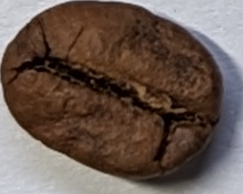
\includegraphics[height=0.8\linewidth, keepaspectratio]{
			./figures/methodology/quaker-bean
		}
		\subcaption{''Quaker``} \label{fig:quakerBeanSingle}
	\end{subfigure}
	\begin{subfigure}
	{0.2\textwidth}
		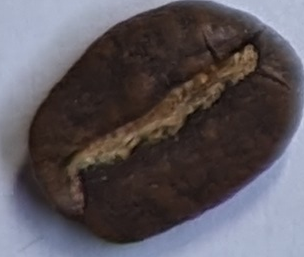
\includegraphics[height=0.8\linewidth, keepaspectratio]{
			./figures/methodology/normal-bean
		}
		\subcaption{Normal} \label{fig:normalBeanSingle}
	\end{subfigure}
	\begin{subfigure}
	{0.2\textwidth}
		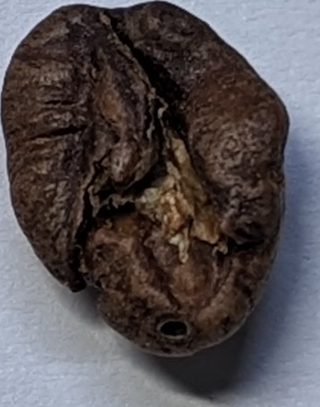
\includegraphics[height=0.8\linewidth, keepaspectratio]{
			./figures/methodology/insect-damaged-bean
		}
		\subcaption{Insect \\ damage} \label{fig:insectBeanSingle}
	\end{subfigure}
	\begin{subfigure}
	{0.2\textwidth}
		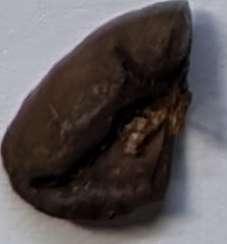
\includegraphics[height=0.8\linewidth, keepaspectratio]{
			./figures/methodology/bean-fragment
		}
		\subcaption{Bean \\ fragment} \label{fig:fragBeanSingle}
	\end{subfigure}
	\begin{subfigure}
	{0.25\textwidth}
		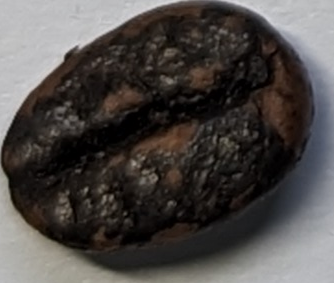
\includegraphics[height=0.8\linewidth, keepaspectratio]{
			./figures/methodology/burnt-bean
		}
		\subcaption{Burnt} \label{fig:burntBeanSingle}
	\end{subfigure}
	\begin{subfigure}
	{0.25\textwidth}
		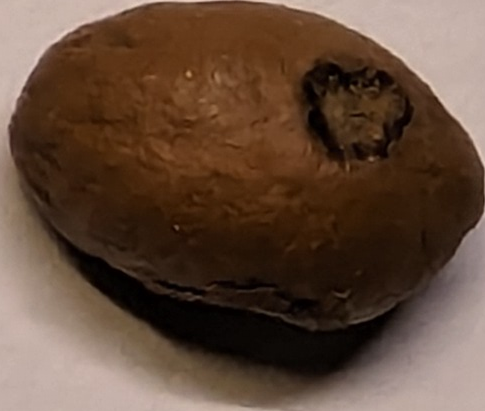
\includegraphics[height=0.8\linewidth, keepaspectratio]{
			./figures/methodology/mold-damaged-bean
		}
		\subcaption{Mould damage} \label{fig:moldBeanSingle}
	\end{subfigure}
	\begin{subfigure}
	{0.25\textwidth}
		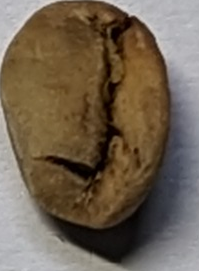
\includegraphics[height=0.8\linewidth, keepaspectratio]{
			./figures/methodology/under-bean
		}
		\subcaption{Underroasted} \label{fig:underBeanSingle}
	\end{subfigure}
	\caption{Examples of bean defects}
	\label{fig:beanDefects}
\end{figure}

Keeping in line with the project
aims, this section will mainly focus on the defects identified in the beans
contained in the dataset.
Overall, the beans exhibited five various defects, whose
counts and short descriptions are presented in table~\ref{tab:beanDefectCounts}.
Figure~\ref{fig:beanDefects} provides a brief look at the various defects, with more
examples available in appendix~\ref{ch:appendix1}.

\begin{table}[h]
	\centering
	\begin{tabular}{|p{0.25\linewidth}|p{0.6\linewidth}|p{0.15\linewidth}|}
		\toprule \textbf{Defect name} & \textbf{Visual features}                                                                                                                                             & \textbf{Count} \\
		\midrule Normal bean          & Even colour, brown to dark-brown hue, no surface damage or blemishes and a round shape with no deformities                                                           & 1311           \\
		Quaker                        & Light brown to brown hue (due to less caramelisation of sugar), scorch marks, brown spots on surface.
		Occasionally, a shrivelled, uneven look of the outside surface & 978            \\
		Bean fragment                 & Significantly deformed or chipped exterior, smaller bean pieces                                                                                                      & 296            \\
		Underroasted                  & Very light brown exterior, dark green or yellow in extremely underroasted beans                                                                                      & 104            \\
		Burnt                         & Dark brown to black exterior, significant scorching or an oily, shiny surface                                                                                        & 50             \\
		Insect/mould damage           & Small, round holes or larger ''craters`` on the surface                                                                                                              & 47             \\
		\bottomrule
	\end{tabular}
	\caption{Bean defect counts}
	\label{tab:beanDefectCounts}
\end{table}

The beans in the dataset belonged to a total of nine varieties and have been processed using six different methods.
The number of beans belonging to each processing method and variety method is shown
on figures~\ref{fig:beanProcessingCounts} and~\ref{fig:beanVarietyCounts} respectively.
\begin{figure}[h]
	\centering
		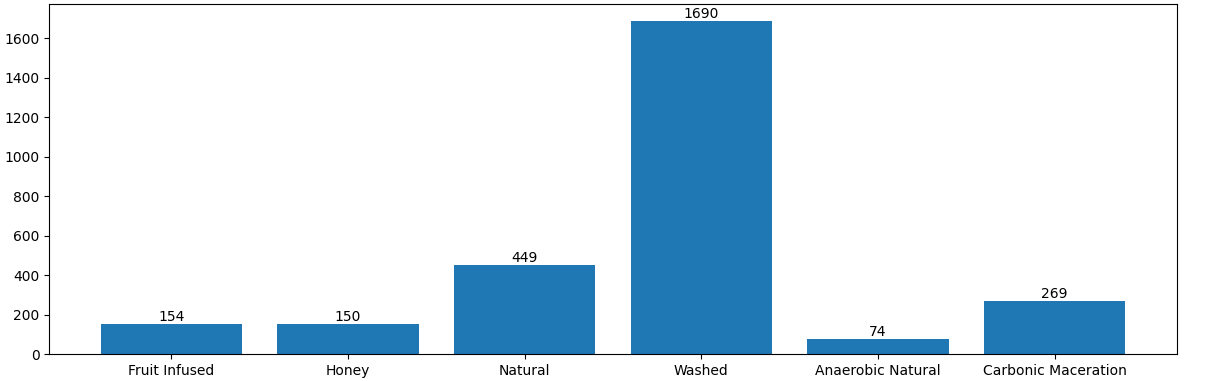
\includegraphics[width=\linewidth, height=2.5cm, keepaspectratio]{
			./figures/methodology/processing-counts
		}
	\caption{Bean processing method counts}
	\label{fig:beanProcessingCounts}

	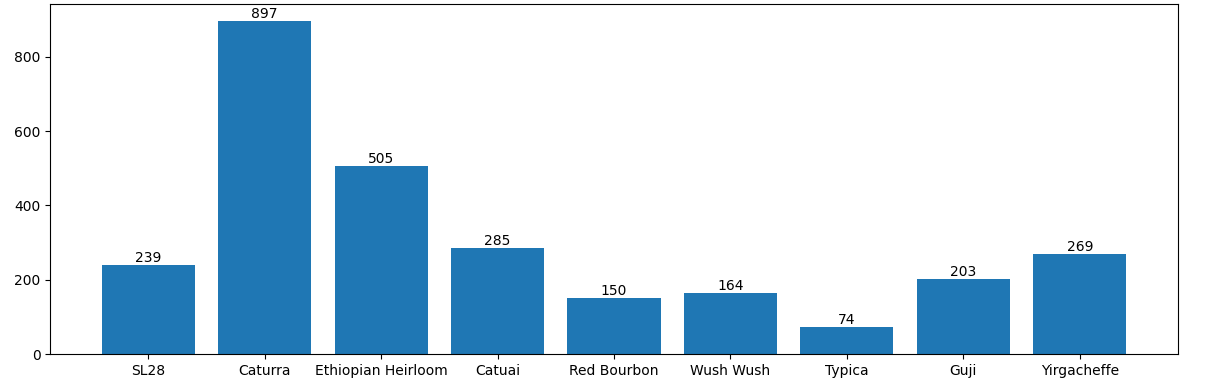
\includegraphics[width=\linewidth, height=2.5cm, keepaspectratio]{
			./figures/methodology/variety-counts
		}
	\caption{Bean variety counts}
	\label{fig:beanVarietyCounts}
\end{figure}

It should be noted that the original intent was for the insect and mould damage to be distinct classes,
however, these defects are quite rare, especially with the higher-grade green coffee the local roasters worked with.
Because of this lack of available data, it was decided to merge the classes: not only do the visual features of the two
defects resemble each other, but the effects they have on the final product are also similar.
While future work could seek an improved dataset and a higher granularity of classes, the merging of the two classes here
is unlikely to reduce the practical usefulness of the classifier in a roaster's daily tasks.
\subsection{Data pre-processing}
\label{subsec:data-pre-processing}
As described in the above section, the beans were arranged in grids when their pictures were taken.
To train the classifier however, each bean had to be contained in its own image, requiring the use of a software solution
to automatically separate each bean.
The solution was implemented in Python and depended heavily on the OpenCV library~\cite{opencvLibrary}, which provides
tools for working with and processing images.

Separating the grid images involved several steps.
First, the image was loaded and converted to grayscale using a built-in OpenCV function.
Then, a threshold was applied to the resulting images to provide a binary separation between the beans and the background.
An important step was inverting the thresholded images so that the background was represented by black pixels
and the beans by white ones - this was required for the contour finding step that followed.

Once the binary images were produced, the \verb |findContours| function was used to identify the contours and
bounding rectangles of each individual bean.
At this stage, additional checks were conducted to ensure that no dust or foreign objects were captured by the algorithm:
bounding rectangles whose areas were uncharacteristically small or large or whose aspect ratio was too imbalanced were rejected.
The expected dimensions were gathered by running the algorithm once and inspecting the produced images: the images tended
to be around 200--400 pixels wide/tall, with an aspect ratio not exceeding 1:3.
Finally, the batch images were separated into sections matching the positions and dimensions of each bounding rectangle.
The resulting images were named reflecting the bean's variety, origin, processing method and defect class and sorted into folders
named in the same pattern.
A CSV file reflecting the class annotations has also been generated and stored in the image directory.
Each row in the CSV file corresponded to a single bean, with the columns containing the image name and the
aforementioned class information.

A visualisation of the data processing pipeline is shown on figure~\ref{fig:imgProcessing}.

\begin{figure}[h]
	\centering
\begin{tikzpicture}
	\node (raw)
		{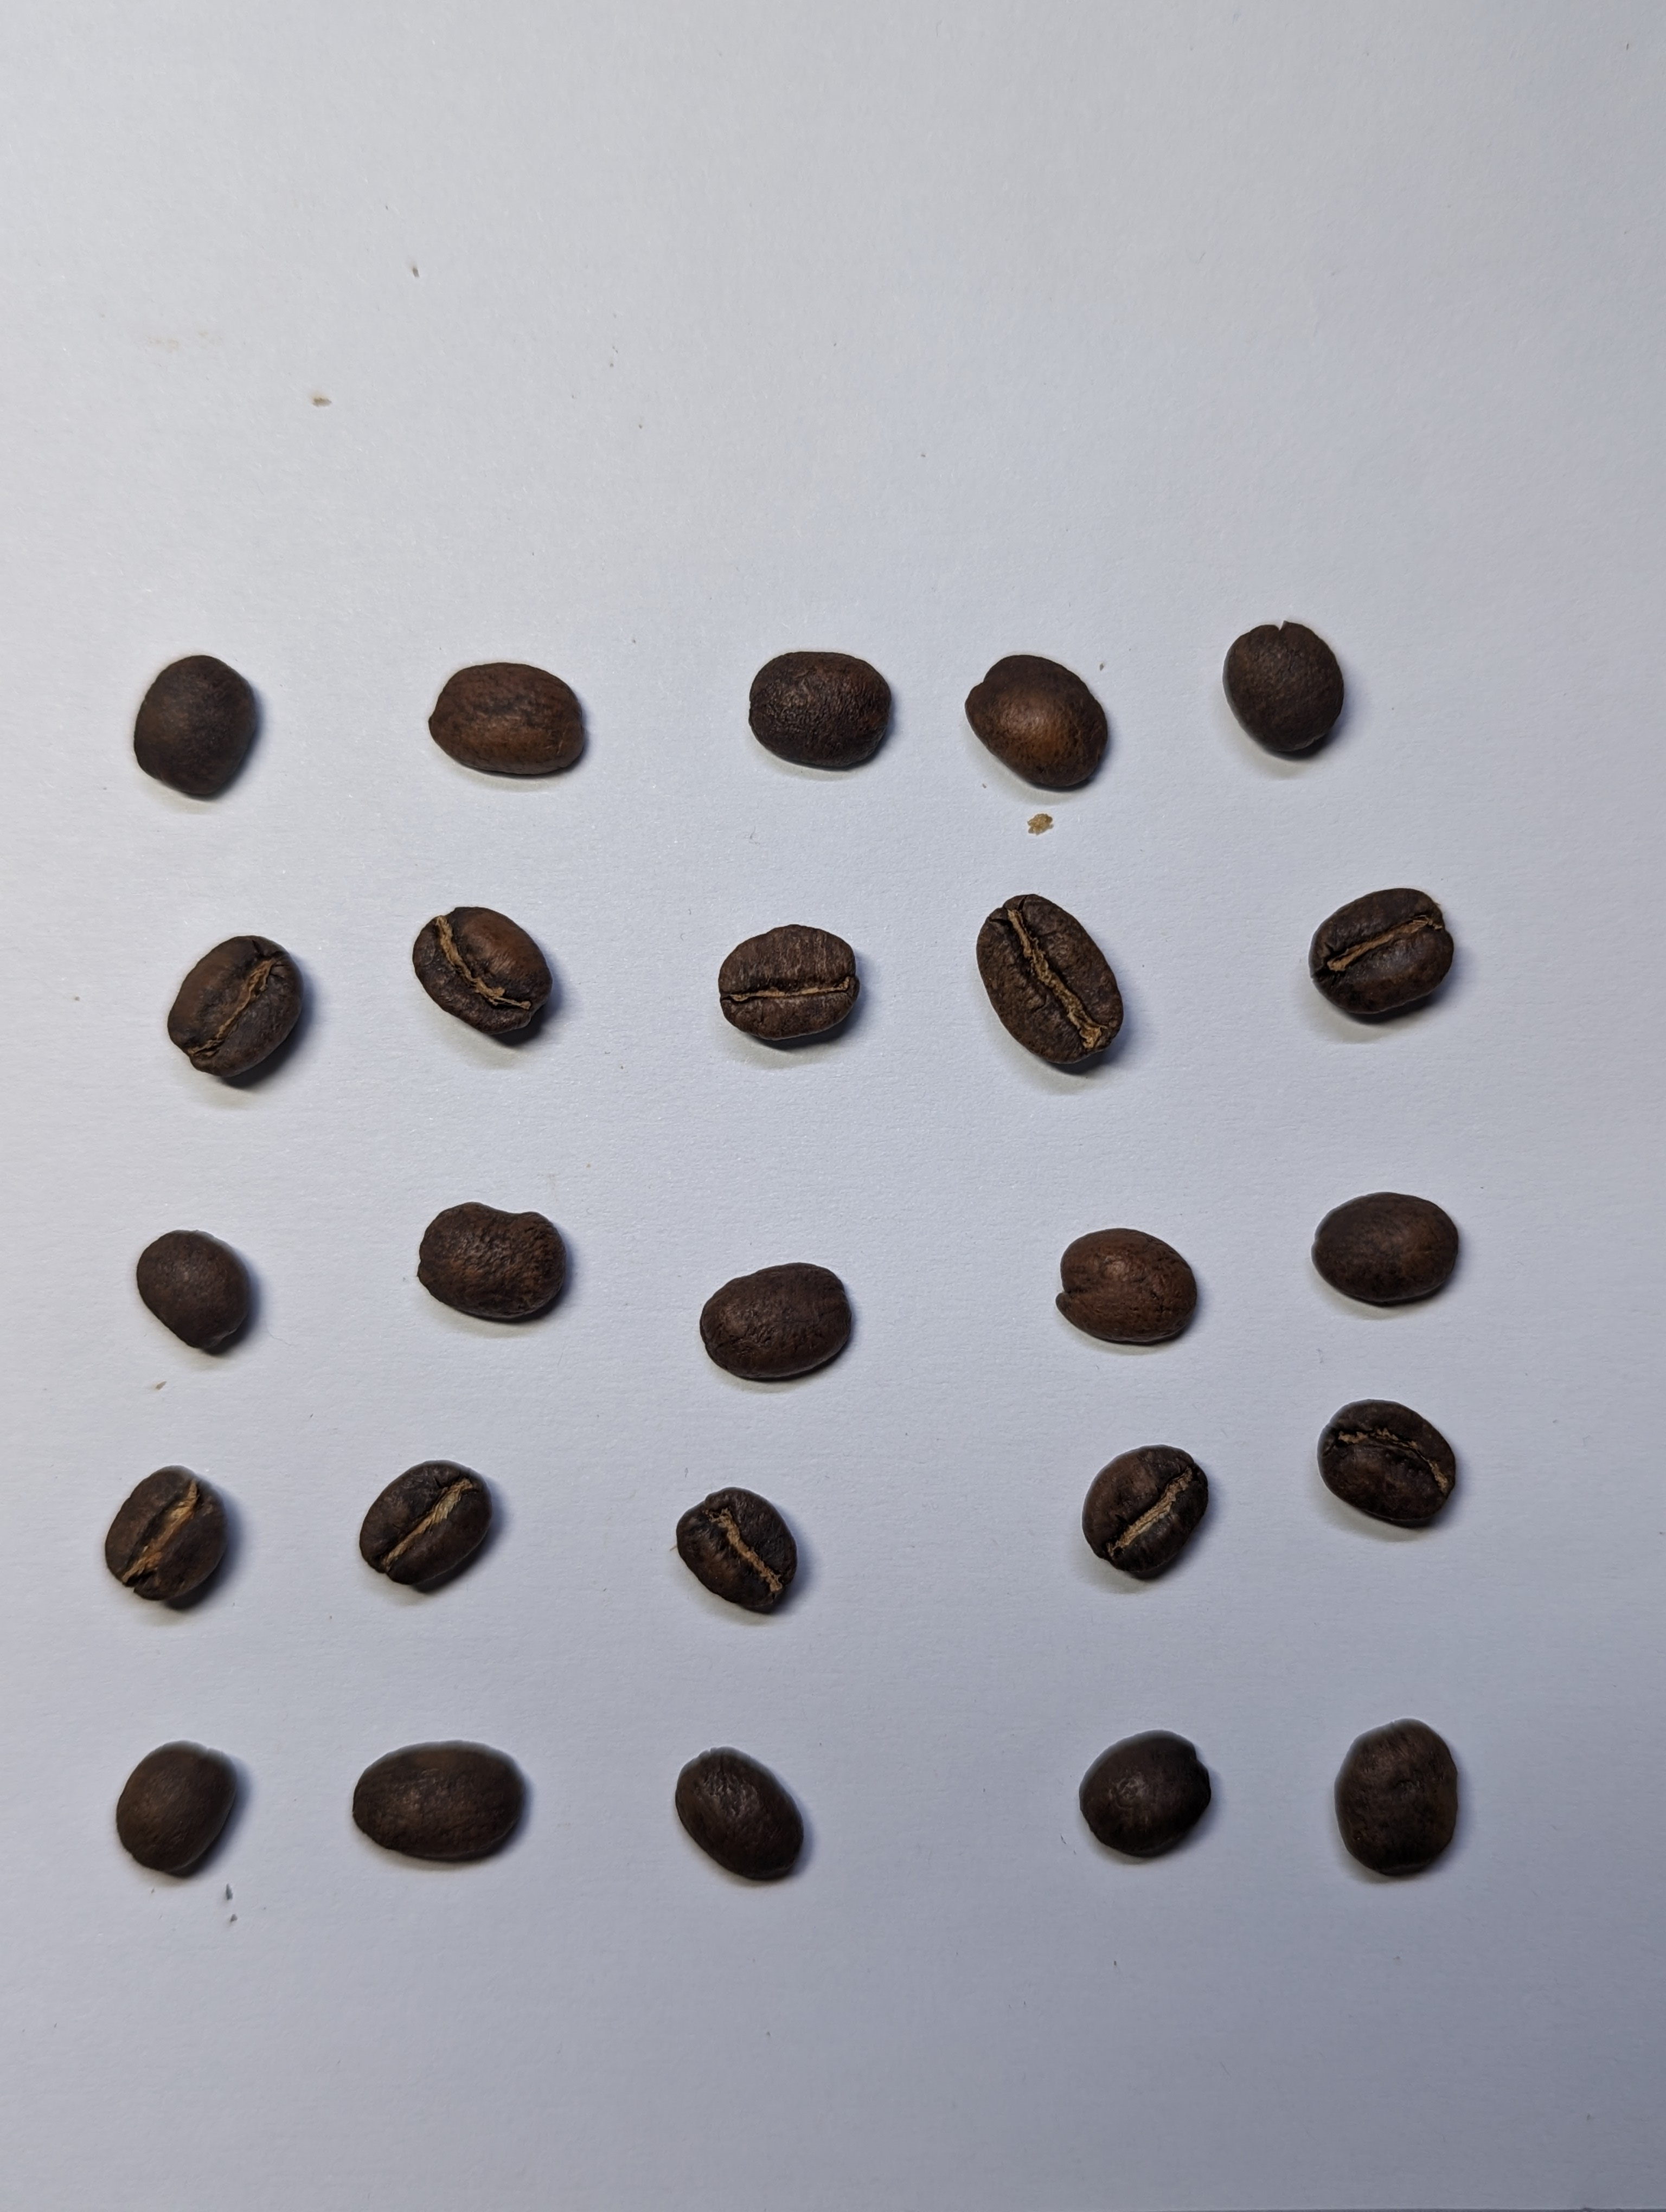
\includegraphics[height=4cm, keepaspectratio]{methodology/bean-batch-raw}};
	\node[right=of raw](gray)
		{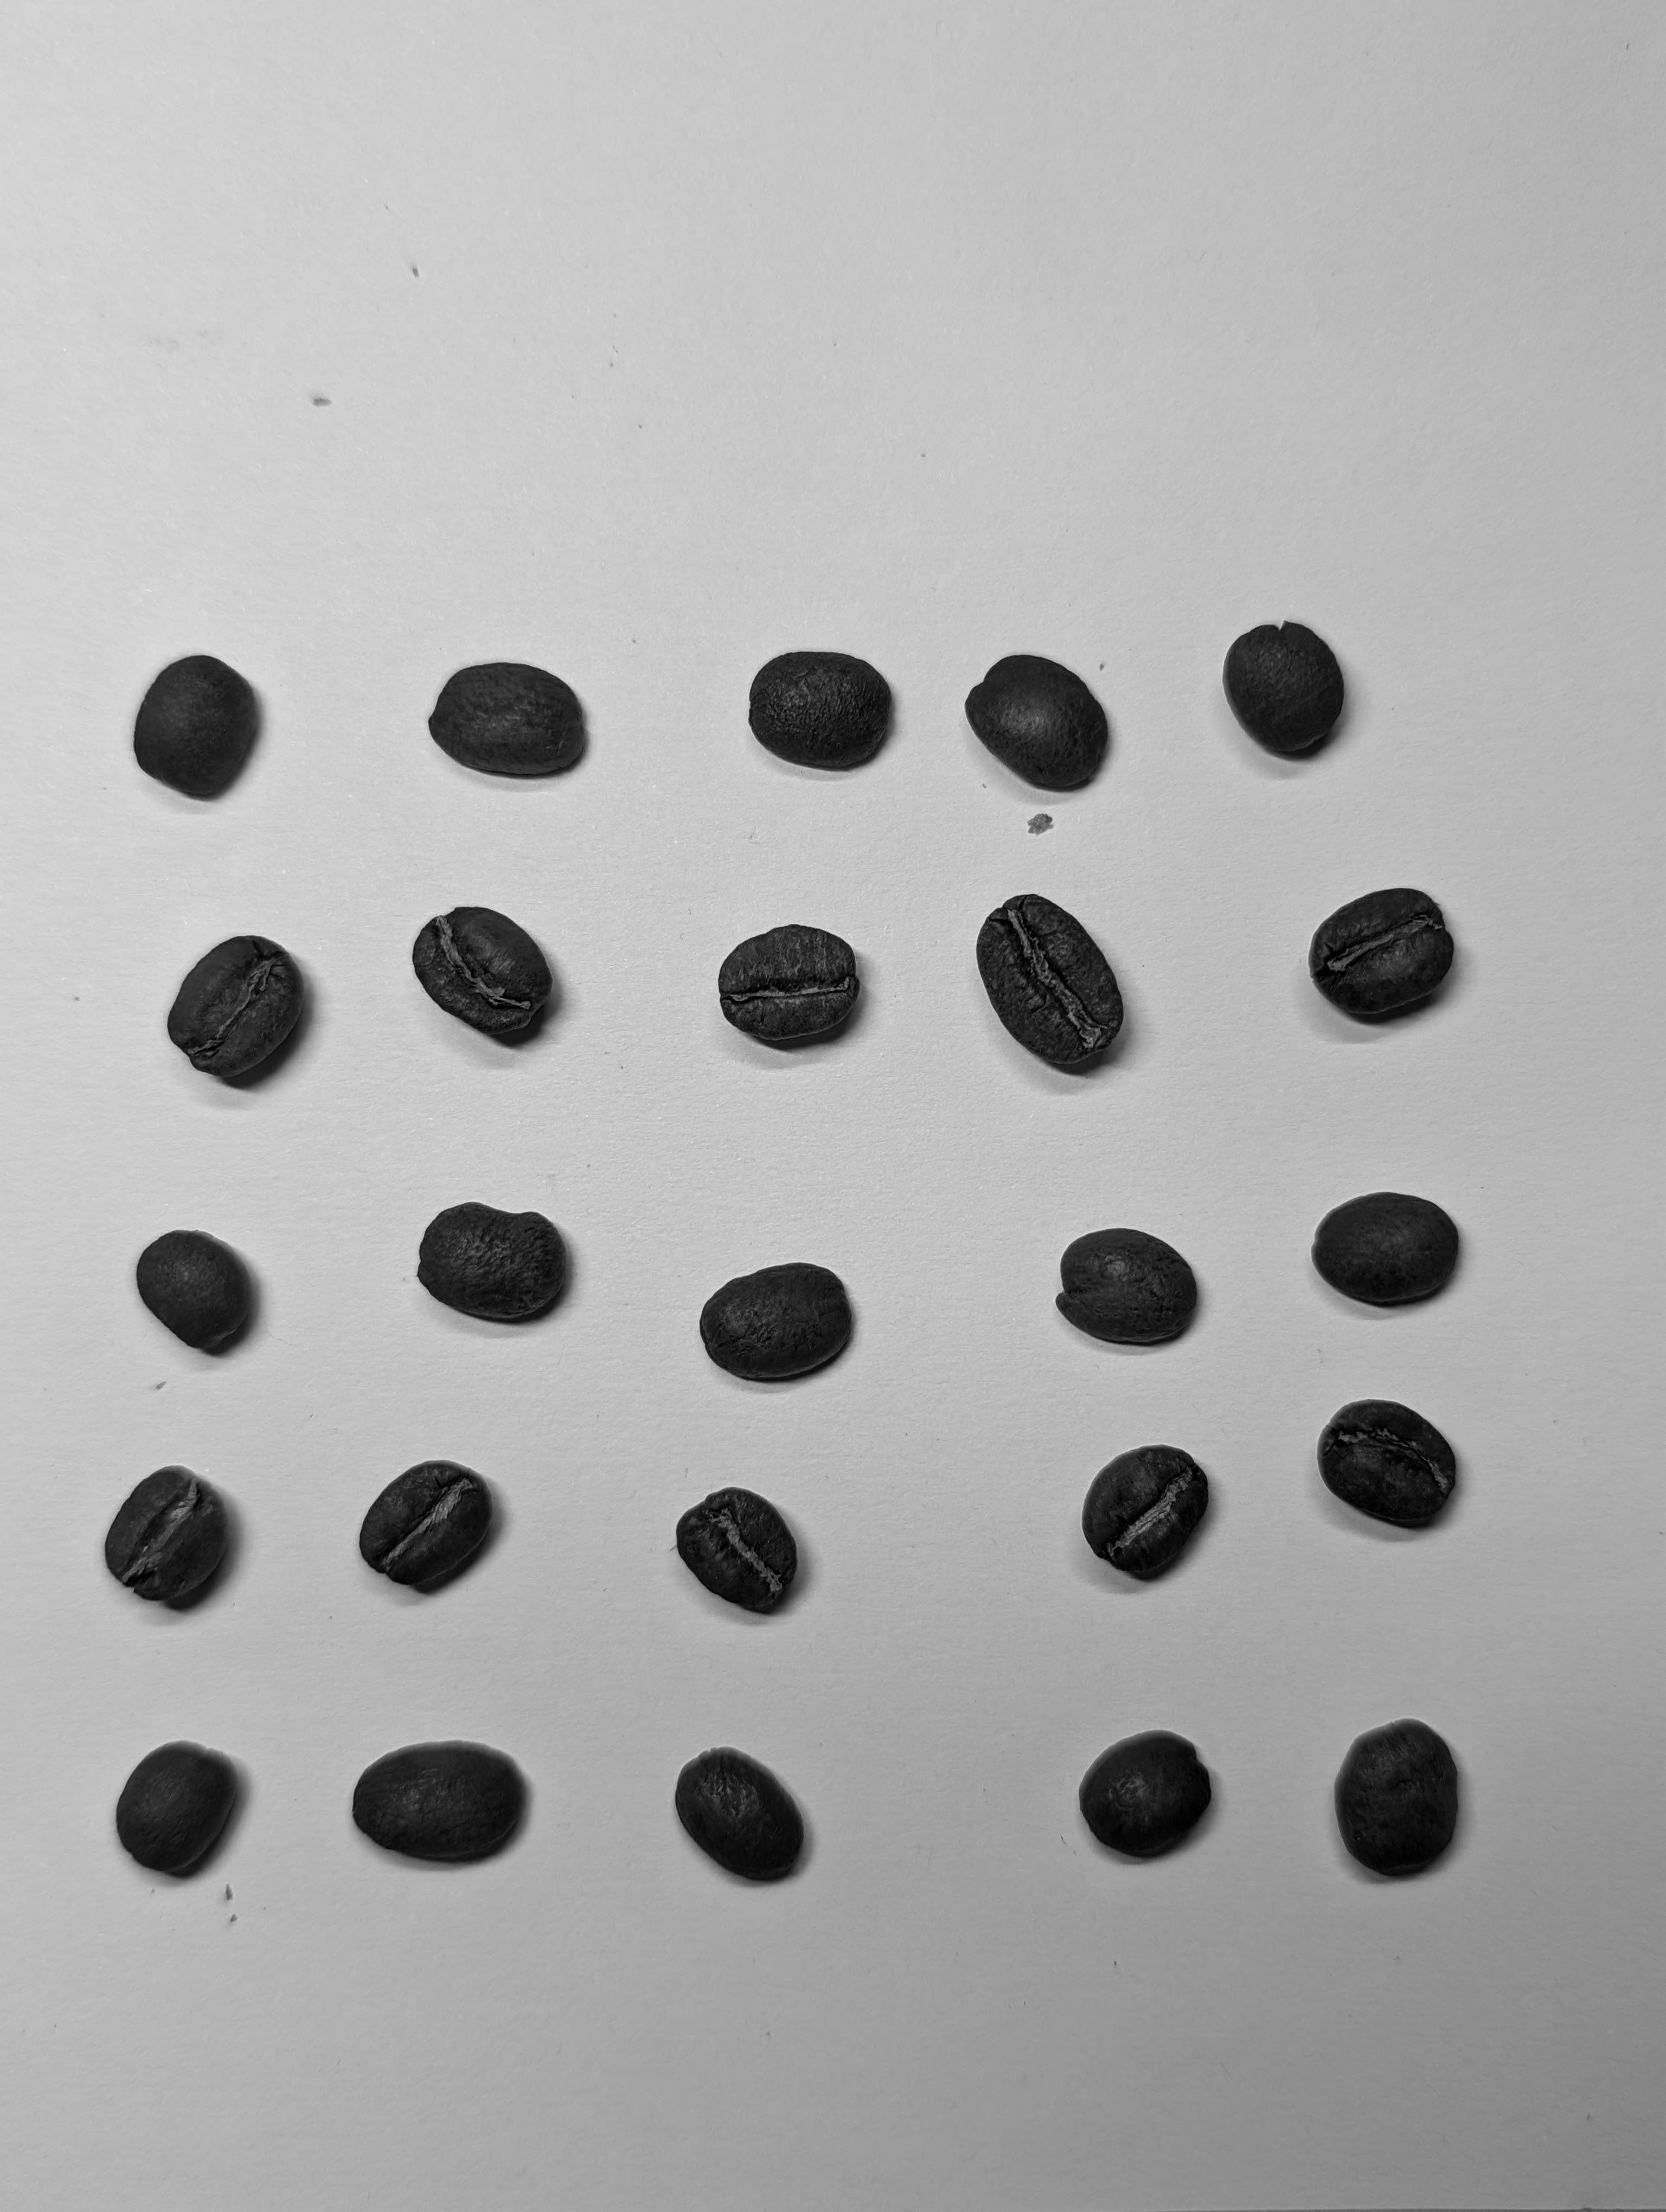
\includegraphics[height=4cm, keepaspectratio]{methodology/bean-batch-gray}};
	\node[below=of gray] (thresh)
		{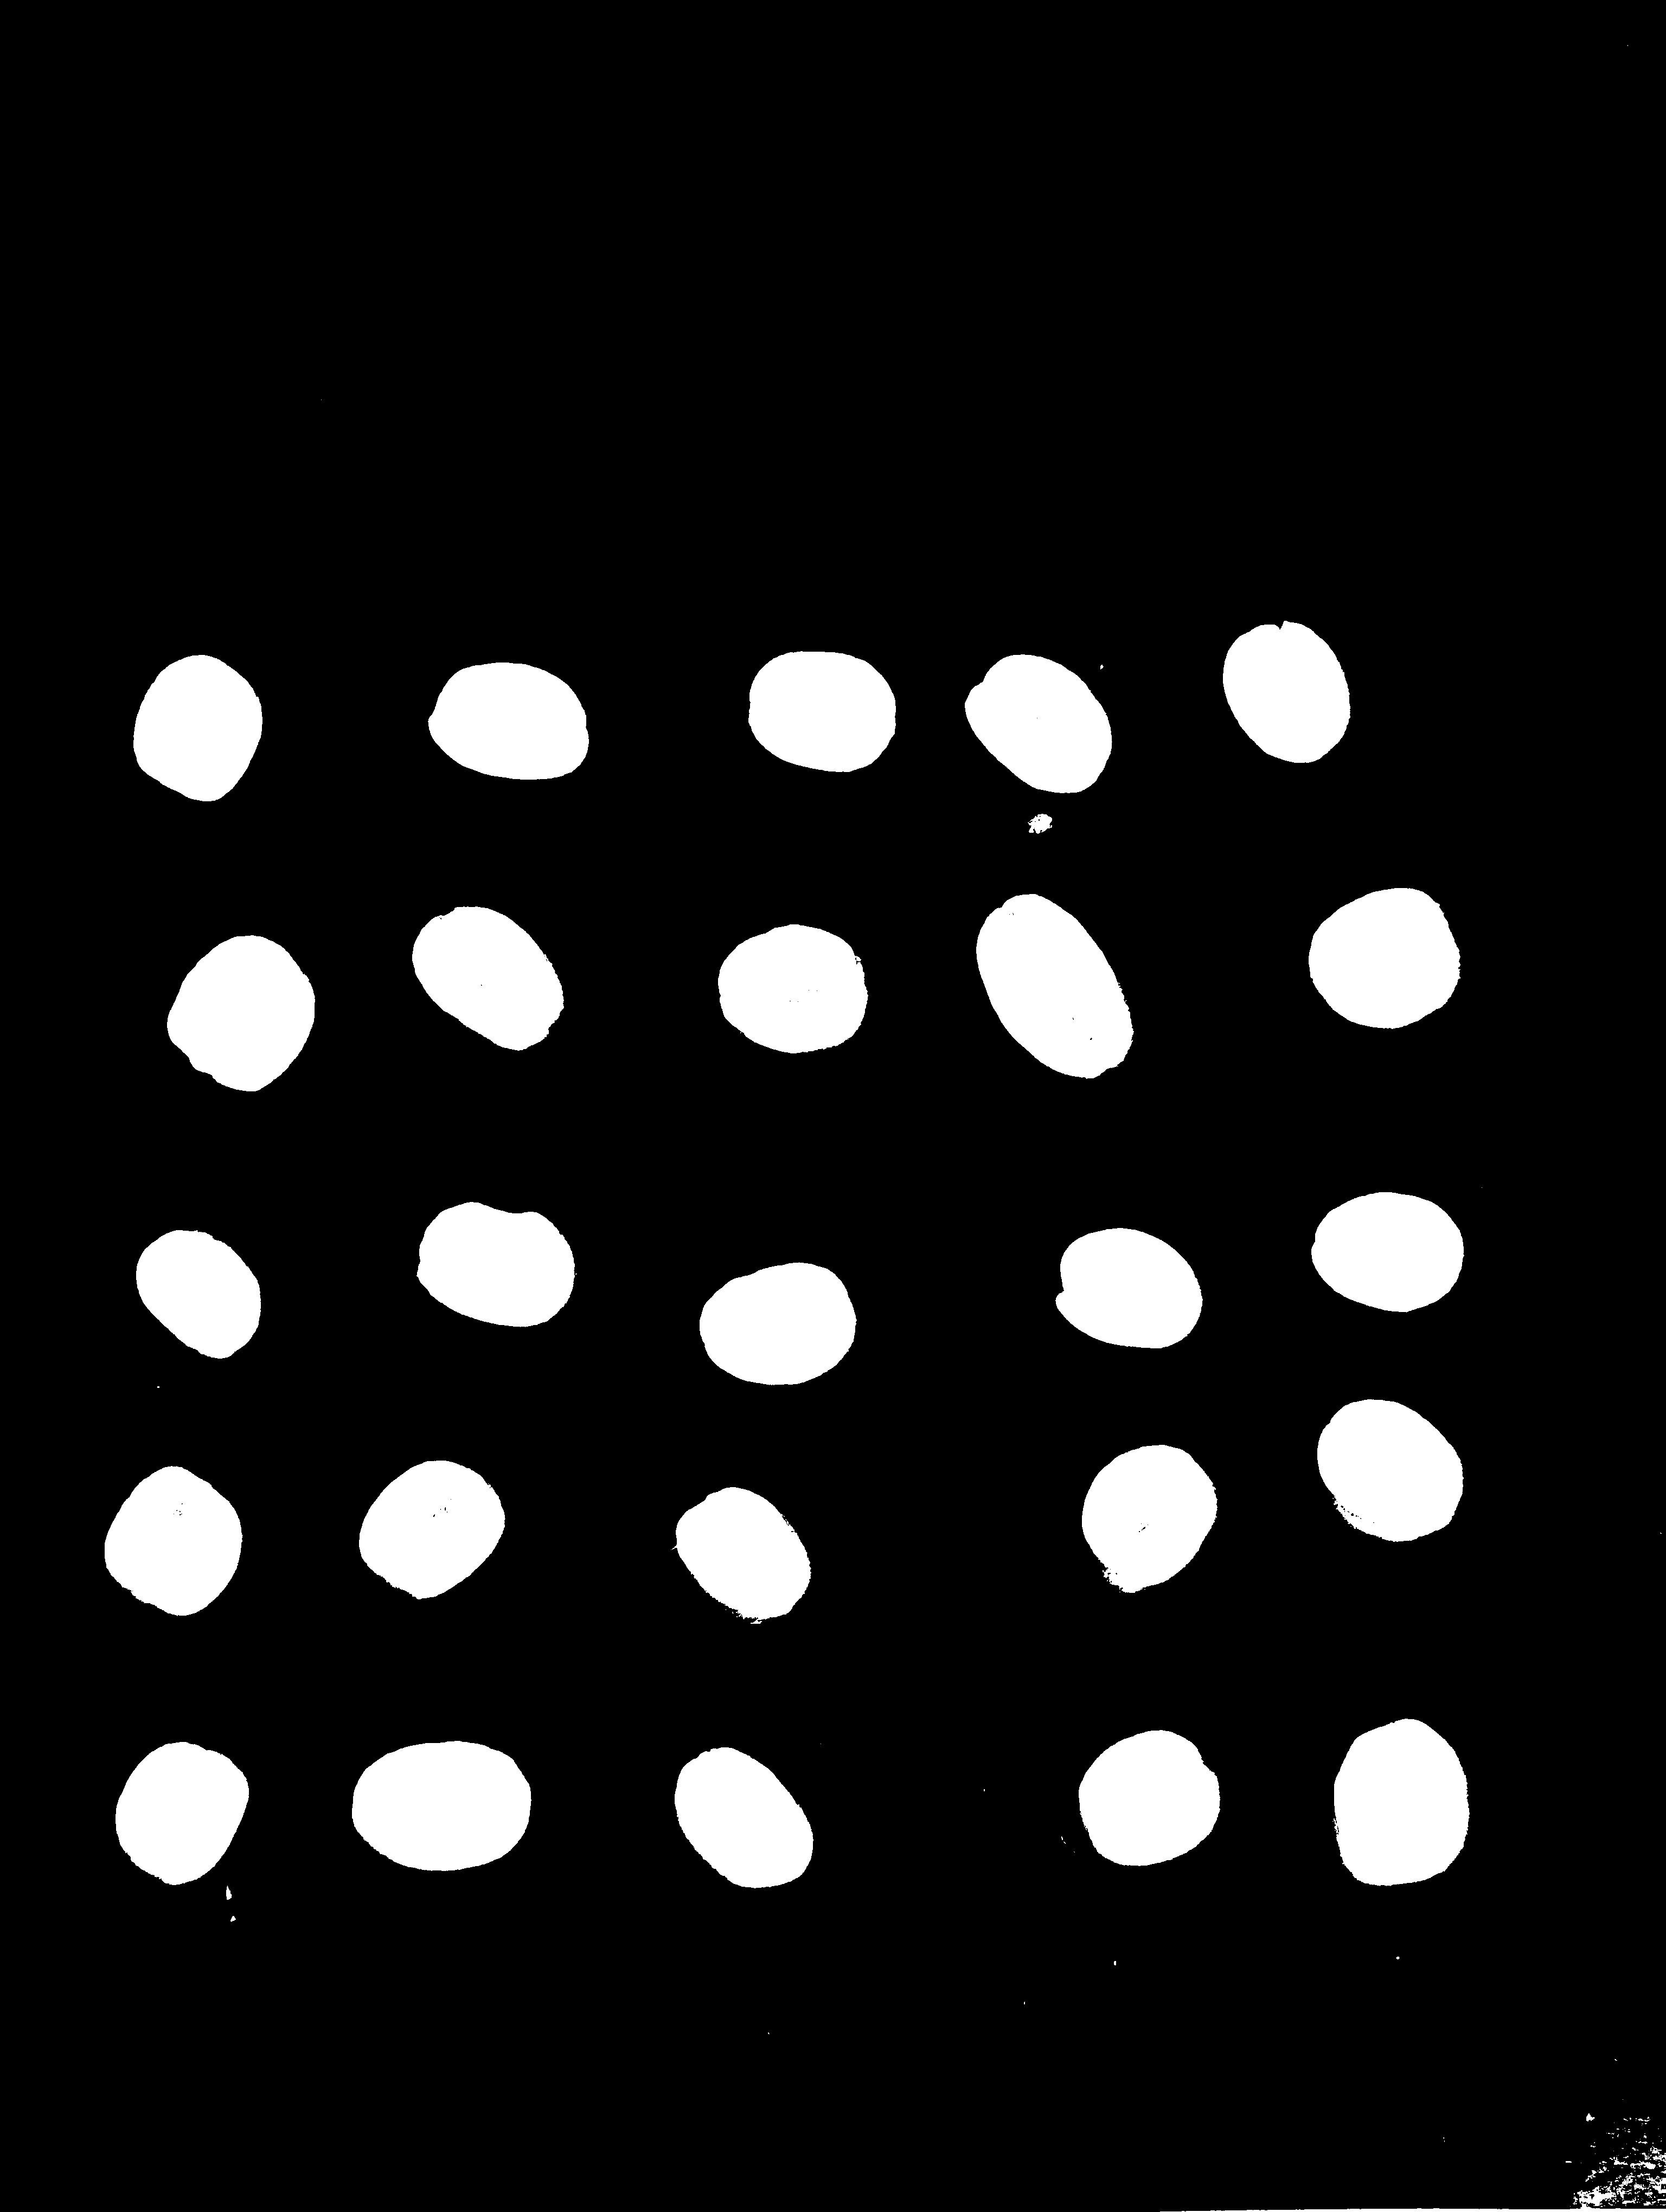
\includegraphics[height=4cm, keepaspectratio]{methodology/bean-batch-thresh}};
	\node[left=of thresh, below=of raw] (contours)
		{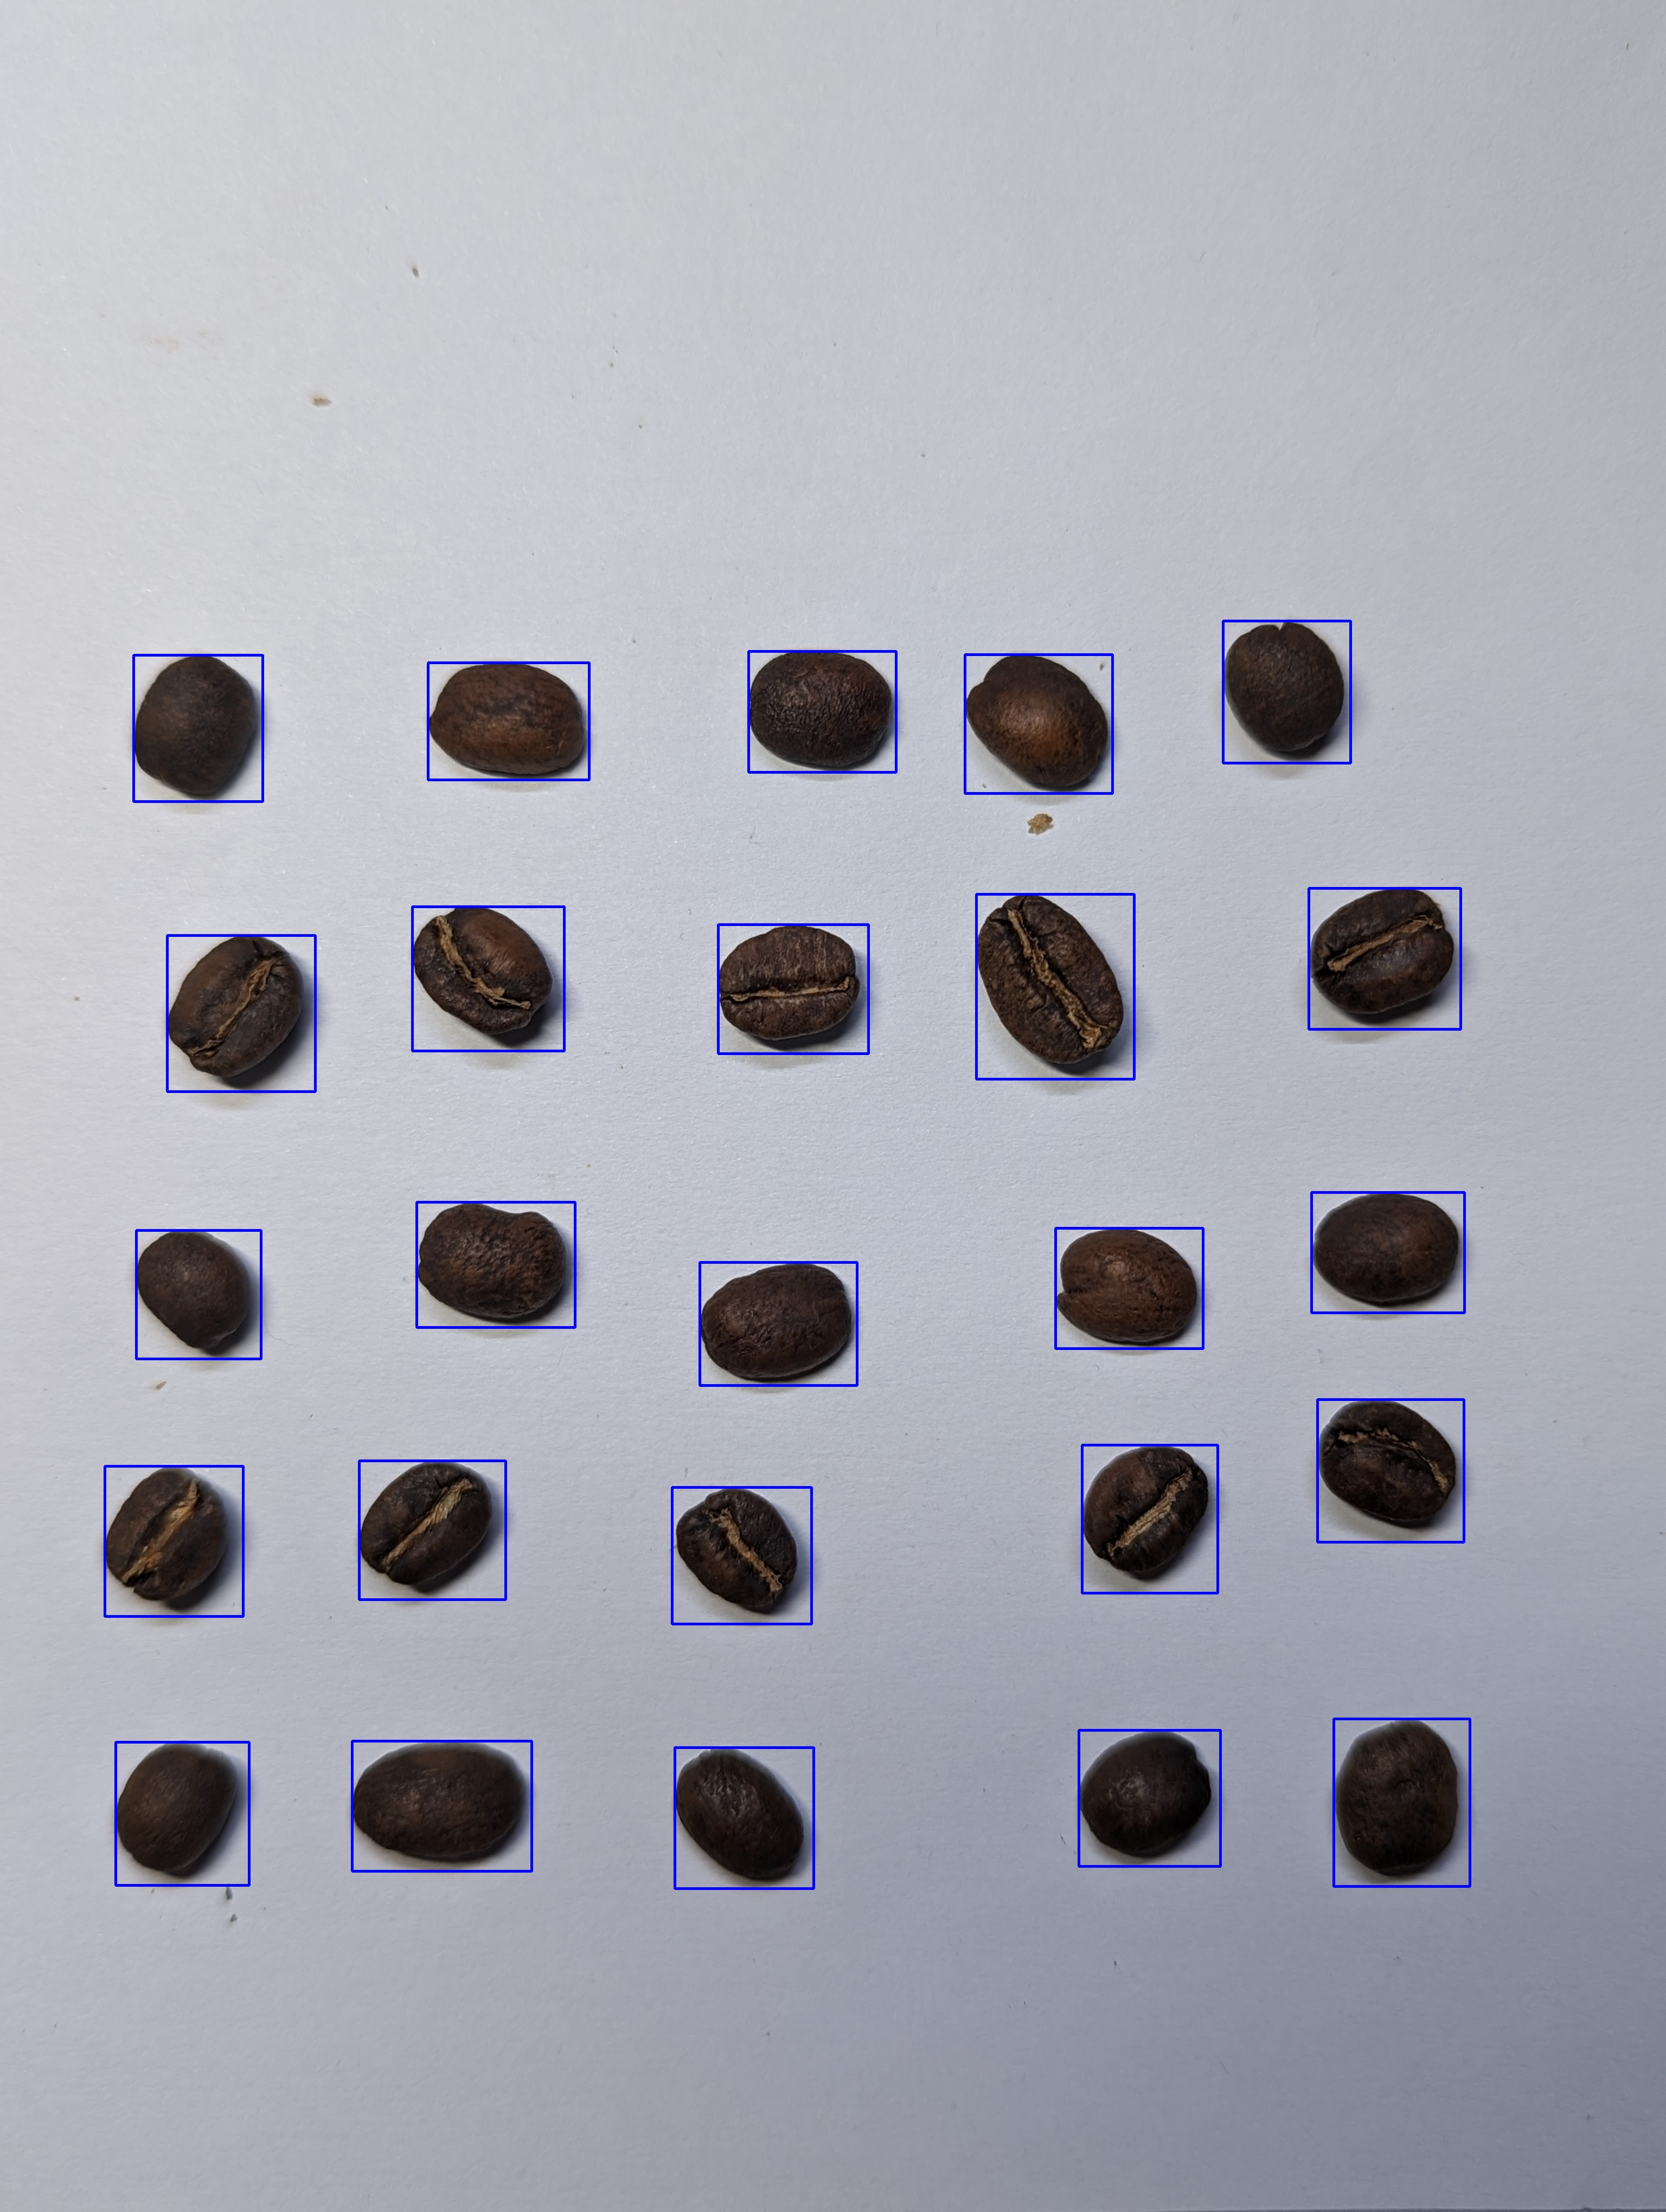
\includegraphics[height=4cm, keepaspectratio]{methodology/bean-batch-contours}};

	\draw[->,thick] (raw) -- (gray);
	\draw[->,thick] (gray) -- (thresh);
	\draw[->,thick] (thresh) -- (contours);
\end{tikzpicture}
	\caption{Image processing pipeline}
	\label{fig:imgProcessing}
\end{figure}

It should be noted that preliminary experiments led to another addition to the image processing steps:
it was found that better performance was achieved when the natural background of the images was replaced with pure white pixels.
To achieve that, the thresholded images were used to manually set all non-bean (i.e. black) pixels to a value of (255, 255, 255),
resulting in a pure white background.
Both versions of the datasets were retained and used in classifier training.

Overall, the data processing pipeline yielded a dataset containing the individual images in a nested directory, with
a CSV annotations file in the top-level directory to be used by a machine learning framework.

\section{Approaches to model development}
\label{sec:approaches-to-model-development}
The following section outlines the approaches taken in implementing a suite of image classifiers for bean defects.
The classifiers were implemented in Python, and, where applicable, were trained on an M3 Apple Silicon system with 36GB
of memory.

The literature review identified 3 general paths that one could take when developing a classifier, each with a different
set of strengths, weaknesses, and aiming to address different priorities.
The following subsection will discuss the approach taken to develop the three models to be evaluated further, in an
increasing order of complexity.
\subsection{Nearest-neighbor classifier}
\label{subsec:knn-classifier}
The primary reasoning behind implementing a KNN-based classifier is its speed of deployment, simplicity of implementation
and good accuracy potential.
As a concept, KNN can be easily understood even by non-technical stakeholders and requires little experimentation apart
from picking the value of K, determining how many ''neighbors`` each input has to be compared against.

One of the main challenges with KNN is its computational cost: the number of comparisons grows quickly with an increase
in the amount of features, dimensions and data points.
Therefore, with the dataset's images containing tens of thousands of pixels, each with three colour channels, a brute-force
approach was dismissed.

An approach seen, among others, in Olivieri et. al.'s paper~\cite{hyperspectralGreenOliveri}, is dimensionality reduction,
which aims to extract the features of the data that contribute to its difference the most.
While several dimensionality reduction techniques exist, the significant visual differences across the bean classes suggested
that the use of colour histograms could efficiently reduce the size of the data while still preserving its differences.

A colour histogram is a relatively simple plot of the distribution of colours in a given image.
A strength of this approach is its resilience to the orientations of beans in the images - the colour distribution stays
the same no matter how the bean is positioned (apart from the small discrepancies in shadows).
Furthermore, by controlling the amount of distinct colours in the histogram, the dimensionality can be easily changed to
make sure there is plenty of data to compare the images by.

It should be noted that the method is not without its criticisms: while colour makes up a significant amount of the difference
between the beans, properties like texture and shape are removed by the dimensionality reduction process.
Also, the size of the image itself can skew the distribution simply due to the difference in the numbers of pixels.

Another approach to a KNN classifier was tested in a preliminary experiment:
there, the images were converted into long vectors by extracting colour information from each channel (red, green or blue)
and concatenating the three resulting grids into a one-dimensional representation.
While this approach was able to correctly classify some images, especially those belonging to the ''normal`` and ''quaker``
classes, the performance on the smaller classes combined with the long prediction times suggested that the colour histogram
provided a better compromise between the richness of the data and the practicality of the classifier.

The best hyperparameters were found in a grid search, with different choices of the value of k, the distance metric
and nearest neighbour calculation algorithm trialed.
In every experiment, the classifier was fitted with 80\% of the data, chosen at random and evaluated on the rest of the data,
with metrics such as overall accuracy, per-class precision, recall and f1 score recorded and tracked.
To maintain a consistent ratio of beans of different types, a stratified split function has been used.

The classifiers and their evaluation were implemented using the Scikit-learn library \cite{sklearnLibrary}, with the calculation of colour
distributions provided by the Scikit-image library \cite{skImageLibrary}.
Loading the data was done by creating a \verb|DataLoader| class provided by the PyTorch library \cite{pytorchLibrary}, which allowed
for the data loading to be easily shared between this classifier and ones developed later.
\subsection{Compact CNN classifier}
\label{subsec:deep-learning}
The aims in developing this classifier were centered around addressing the weaknesses of the one described above,
namely its high prediction cost and its lack of ability to extract complex features from input images.

For this, a convolutional neural network (CNN) was selected as a design candidate, based on their
efficiency at classifying images and common use in industry.
Furthermore, the principles behind the functionality of convolution layers suggest that the high resolution of the input
images would be a benefit, with the classifier being able to extract texture and shape information from each image.

While countless network architectures exist, the goal with this classifier was ensuring the smallest possible classification time,
and, therefore, smaller designs were considered.
The MobileNet V2 architecture~\cite{mobileNet} stood out for its relatively small number of parameters and a promised ability to run even on
a mobile device.
Therefore, a high performance result from such a small architecture would result in a classifier that is able to be deployed
on any system, removing the cost barrier between coffee roasters and automatic quality control methods.
Furthermore, a smaller architecture would be faster to train on a custom dataset, providing greater flexibility.

Other smaller architectures such as ShuffleNet V2`~\cite{shuffleNet} were considered and trialled in preliminary experiments,
however, MobileNet consistently outperformed the others and was therefore selected as the final model of this type.
\subsection{Application of transfer learning to large models}
\label{subsec:transfer-learning}
The models trialled in this set of experiments were the largest in terms of the number of parameters and
architectural complexity.
The idea behind using these models was that the large number of parameters could allow them to extract even more information
from the input images and gain better performance, especially in smaller classes.

A drawback of such large modules is their need for large dataset during training, a requirement which the gathered data would
struggle to fulfil.
To overcome this limitation, a technique called transfer learning was employed.
In this technique, the model is first trained on a large, not necessarily domain-specific dataset and then
''fine-tuned`` on a smaller selection of domain-specific data.
This technique allows the models to learn to extract features from images and then sharpen that knowledge by training on a dataset
specific to the given task.

A commonly used general-purpose dataset is ImageNet~\cite{imageNet}, containing over a million images belonging to a thousand
classes.
Pre-trained models were loaded from the \verb|torchvision.models| package provided by PyTorch~\cite{pytorchLibrary}.

One of the more promising architectures was ResNet~\cite{resNet}, with a deep architecture boasting a high top-1 accuracy on the imageNet dataset.
Several versions of the ResNet architecture exist, with the 18, 34 and 50 layer versions trialled in the experiments.

Other tested architectures included the EfficientNet V2~\cite{efficientNet} and the Swin transformer~\cite{swinTransformer},
which were selected for their reported accuracy on the imageNet dataset.

An important step in this set of experiments was the readjusting of the model before making predictions on the bean dataset:
since all models were tailored to ImageNet, the number of output neurons in their final fully-connected layers was mismatched.
The fixes involved inspecting the models' architectures, identifying the attribute name of the final layer, and replacing it with an
instance of the \verb|torch.nn.Linear()| class, where the number of input neurons matched that of the old fully connected layer,
and the number of outputs was equal to the number of classes in the dataset.

	\chapter{Results}
	\label{ch:results}
    \section{Loading and pre-processing the dataset}
\label{sec:loading-and-pre-processing-the-dataset}
As mentioned in section~\ref{subsec:data-pre-processing}, a PyTorch \verb|DataLoader| was used to label and load the images
for each classifier.
After the images were loaded, they were resized to the same $400 \times 400$ resolution, ensuring that most images are
enlarged rather than shrunk.
This was a conscious choice, as the textural features of some defects were quite small and harsh shrinking of the images
could have corrupted or outright removed that information.

After the images were set to a consistent size, the further processing differed slightly between the classifier types:
for the KNN classifier, no further processing was done.
This decision was based on the reasoning in section~\ref{subsec:knn-classifier} and aimed to preserve the colour values of the pixels.
For neural network-based classifiers, the processing consisted from a sequence of transforms from the Pytorch \verb|torchvision.transforms|
package and consisted of the following items:
\begin{itemize}
    \item Converting the images to the \verb|float32| data type to enable training on the M3 GPU cores
    \item For the training set, applying a random horizontal flip and a rotation to augment the dataset
    \item For the testing set, only applying a rotation to augment the test data due to its small size
\end{itemize}

After applying a stratified train/test split, with 80\% of images used for training, the class counts for the two sets are
shown in table~\ref{tab:finalTrainTestClassCuts}.
The split was applied with a constant random state value for repeatable results.
\begin{table}[h]
    \centering
    \begin{tabular}{lll}
        \toprule
        \textbf{Defect name} & \textbf{Training count} & \textbf{Testing count} \\
        \midrule
        Normal & 1048 & 263 \\
        Quaker & 782 & 196 \\
        Bean fragment & 237 & 59 \\
        Underroasted & 83 & 21 \\
        Burnt & 40 & 10 \\
        Insect/Mould & 38 & 9 \\
        \bottomrule
    \end{tabular}
    \caption{Finalised training and testing set class counts}
    \label{tab:finalTrainTestClassCuts}
\end{table}

As seen from the the above table, despite the initial aims of the project, the distribution of the classes was quite unbalanced.
While no ill effect on the KNN performance has been observed, such a skewed distribution is highly likely to negatively
affect the performance of a neural network due to the low chance of a smaller class' sample being picked in a given epoch.

While Pytorch provides facilities for sampling from a given list of indices and sampling with a manually set probability for each class,
there is no built-in method for combining the two, making it difficult to apply a weighted sampler to a subset of the total dataset.
The solution to this problem was found in a third-party library~\cite{imbalancedSampler} providing the \verb|ImbalancedDatasetSampler| class.
This sampler draws from a given list of indices with the probability of each class' sample being picked equal to
$P(Class_{sample} = C) = \frac{1}{\arrowvert\{x \in X \colon Class_x = C\}\arrowvert}$ for class $C$ and dataset $X$.

Overall, by combining the techniques of over and under sampling as well as data augmentation, the networks were able to learn on a relatively
evenly balanced and varied dataset.
\section{KNN classifier results}
\label{sec:knn-results}
The experiments with a KNN classifier followed the methods outlined in section~\ref{subsec:knn-classifier}.
The sets of hyperparameters used to tune the classifier were as follows:
\begin{itemize}
    \item Distance calculation metric $M = \{Euclidean, Manhattan, Canberra\}$
    \item Number of nearest neighbours $K = [1, 30]$
    \item Nearest neighbour calculation algorithm $A = \{KDTree, Brute-force\}$
    \item Number of bins in colour histogram $N = \{32, 64, 128, 256\}$
\end{itemize}

All but the last hyperparameter were added to a set of nested loops with the candidate classifier being initialized with the
chosen values.
The number of bins was set separately as it was applied to the dataset itself prior to fitting the classifier.

The experiments produced two noteworthy classifiers, whose hyperparameter choices and overall accuracy are presented in table~\ref{tab:knnResults}.
\begin{table}[h]
    \begin{tabular}{@{}llllll}
        \toprule
        & \textbf{\makecell{Distance\\metric}} & \textbf{K value} & \textbf{\makecell{Calculation\\algorithm}} & \textbf{\makecell{Histogram\\bin count}} & \textbf{\makecell{Overall\\accuracy(\%)}} \\
        \midrule
        \textbf{KNN-1} & Manhattan & 28 & KDTree & 32 & 75.6 \\
        \textbf{KNN-2} & Canberra & 7 & KDTree & 32 & 75.8 \\
        \bottomrule
    \end{tabular}
    \caption{Finalised KNN classifiers}
    \label{tab:knnResults}
\end{table}

As seen from the above table, both classifiers achieved a relatively high accuracy.
However, inspecting the per-class performance of these classifiers reveals a significant difference.
A metric that can be used to compare per-class performance is the f1-score:
$f_1 = \frac{2tp}{2tp + fp + fn}$, where $tp$, $fp$ and $fn$ are the true positive, false positive and false negative rates respectively.
It should be noted that even the f1 score may not show the full picture: it may be insightful to also look at the precision
($\frac{tp}{tp + fp}$) and recall ($\frac{tp}{tp + fn}$) values per each class.
These metrics for KNN-1 and KNN-2 are presented in table~\ref{tab:knnScores}.
\begin{table}
    \centering
    \begin{tabular}{*7l}
        \toprule
        \textbf{Class} & \multicolumn{3}{c}{KNN-1} & \multicolumn{3}{c}{KNN-2} \\
        \midrule
        {} & Precision & Recall & F1 & Precision & Recall & F1 \\
            \textbf{Normal} & 0.77 & 0.95 & 0.85 & 0.78 & 0.92 & 0.84  \\
            \textbf{Quaker} & 0.73 & 0.83 & 0.76 & 0.74 & 0.81 & 0.77 \\
            \textbf{Bean fragment} & 0.82 & 0.15 & 0.25 & 0.58 & 0.12 & 0.20 \\
            \textbf{Underroasted} & 1.00 & 0.05 & 0.09 & 0.71 & 0.57 & 0.63 \\
            \textbf{Burnt} & 0.00 & 0.00 & 0.00 & 1.00 & 0.30 & 0.46 \\
            \textbf{Insect/Mould} & 0.00 & 0.00 & 0.00 & 0.50 & 0.11 & 0.18  \\
        \bottomrule
    \end{tabular}
    \caption{KNN classifier evaluation metrics}
    \label{tab:knnScores}
\end{table}

The above data suggests that the canberra distance metric allows the classifier to gain better
performance with the under-represented classes, while slightly reducing the performance on larger ones.
This is an important insight, suggesting that the metric can be picked according to the classifier's use case:
the manhattan metric can provide a powerful sorter where one may only be concerned from separating defective and normal beans,
while the canberra metric can provide insights into the distribution of the defects themselves.
It is clear, however, that the colour histogram may not be a powerful enough technique to explain the differences between
the defects and that a more sophisticated solution may be needed if an understanding of defect frequencies (or, an even more accurate sorter)
is the goal.


\section{Compact CNN results}
\label{sec:compact-cnn-results}
Similar to the above section, several model architectures have been tested.
Unlike with KNN classifiers, the hyperparameter space for neural networks is much greater, with many options of loss functions,
optimizer algorithms and more.
This meant that a simple grid search would be incredibly time and resource intensive and that a more thoughtful approach was needed.

The first item considered was the optimizer selection, with the Adam~\cite{adamGrad} and Stochastic gradient descent (SGD) algorithms being
the main candidates due to their wide adoption in industry and strong results on existing datasets.
While both optimizers showed good results when training the models, the SGD optimizer was chosen in the end for its ability
to be customized with momentum (with a value of 0.9 used) and its more intuitive operation.

A loss function needed to be picked next - being a classification problem with multiple classes, binary methods were not applicable,
therefore the choice fell on the binary cross-entropy function, which at a high level, measures the extent to which the
probability distribution of the model's prediction matches that of the actual data.
It should be noted that the Pytorch implementation of this loss function differs slightly from the commonly seen definition,
requiring that the input to the loss function consists of the actual class labels rather than the probability of each class
for each item in a batch for best performance.

Finally, the batch size and epoch number were selected experimentally - initial attempts showed a significant boost in accuracy
(though, at the expense of longer training times) when a smaller batch size was used: switching from 32 down to 8 led
to the biggest increase, with little to no gain seen from further reductions.
The number of epochs was determined from the size of the batches and from observing the magnitude of the changes in the loss function
with the optimal number being 40 for the shuffleNet and mobileNet architectures.

The optimal learning rate for the optimizer was different depending on the number of the current epoch.
While larger ''jumps`` were acceptable and even welcome at the earlier stages, a large learning rate could ruin tens of epochs
of training nearing the end of the training loop.
Therefore, instead of attempting to pick a single learning rate value, a scheduler provided by PyTorch was used.
The chosen solution was an instance of the \verb|StepLR| class, halving the learning rate every 10 epochs for both
ShuffleNet and MobileNet.
Overall, the two selected architectures achieved a significant improvement in both overall accuracy and per-class
metrics over the KNN classifier, with the results presented in table~\ref{tab:cnn-small-scores}.
The total accuracy percentages were 84\% and 81\% for MobileNet and ShuffleNet respectively.

\begin{table}
    \centering
    \begin{tabular}{*7l}
        \toprule
        \textbf{Class} & \multicolumn{3}{c}{MobileNet V2} & \multicolumn{3}{c}{ShuffleNet} \\
        \midrule
        {} & Precision & Recall & F1 & Precision & Recall & F1 \\
        \textbf{Normal} & 0.93 & 0.95 & 0.94 & 0.92 & 0.94 & 0.93  \\
        \textbf{Quaker} & 0.77 & 0.90 & 0.83 & 0.82 & 0.75 & 0.78 \\
        \textbf{Bean fragment} & 0.93 & 0.50 & 0.64 & 0.77 & 0.63 & 0.69 \\
        \textbf{Underroasted} & 0.57 & 0.62 & 0.60 & 0.28 & 0.76 & 0.41 \\
        \textbf{Burnt} & 1.00 & 0.40 & 0.57 & 0.75 & 0.30 & 0.43 \\
        \textbf{Insect/Mould} & 0.50 & 0.11 & 0.20 & 0.00 & 0.00 & 0.00  \\
        \bottomrule
    \end{tabular}
    \caption{Compact CNN evaluation metrics}
    \label{tab:cnn-small-scores}
\end{table}

Overall, moving to a compact CNN has shown a great improvement in both accuracy and per-class metrics over the KNN
classifier.
Despite that, the performance in smaller classes is still somewhat lacking, with the underroasted, burnt and insect damaged
beans being frequently misclassified.
It is clear that the network is lacking information to build a knowledge of the features of these beans from the small
data samples the dataset provides.
The next section will look at addressing these shortcomings by applying transfer learning to a much larger model.
\section{Transfer learning results}
\label{sec:transfer-learning-results}
When selecting the models here, much less concern was given to the size of the model - the main criteria instead were
their performance on a known dataset like ImageNet~\cite{imageNet}.

The ResNet architecture stood out as having great performance on the dataset and a good track record of successful
transfer learning applications.
Several versions of the architecture exist, with 18, 34, 50 and 152 layers.
The first three were selected for experiments, with the extremely large size of the 152 layer version leading to excessively long
training loops and marginal gains over the smaller architectures in preliminary experiments.
For comparison, the MobileNet architecture from the previous section and Swin transformer~\cite{swinTransformer} were also trained,
with the latter serving as an example of a transformer network.

As mentioned in section~\ref{subsec:transfer-learning}, each network was adjusted to predict 6 classes and trained using a similar
iterative approach as described in section~\ref{sec:compact-cnn-results}.

While training the models, it was discovered that they benefited from a lower learning rate and more aggressive scheduling,
with the ResNet models performing best with the learning rate reduced by ten times every eight epochs.
The best performing optimizer and loss function were SGD and Cross entropy loss respectively, though, with slightly different settings
from the ones described in section~\ref{sec:compact-cnn-results}.

It should be noted that MobileNet and ResNet were trained entirely - that is, every weight was updated during training.
The Swin transformer on the other hand, had all its weights frozen (by marking them as not requiring gradient calculations in PyTorch)
except those in the final layer.
This was done as the extreme size of the Swin transformer network caused poorer performance on the smaller classes when all weights were updated -
retaining the weights trained on ImageNet allowed it to better classify the smaller bean categories.

\begin{table}[h]
    \centering
    \begin{tabular}{*{10}l}
        \toprule
        \textbf{Class} & \multicolumn{3}{c}{ResNet 18} & \multicolumn{3}{c}{ResNet 34} & \multicolumn{3}{c}{ResNet 50} \\
        \midrule
        {} & {Prec.} & {Rec.} & F1 & {Prec.} & {Rec.} & F1 & {Prec.} & {Rec.} & F1 \\
        \textbf{Normal} & 0.93 & 0.98 & 0.96 & 0.96 & 0.99 & 0.98 & 0.99 & 0.99 & 0.99\\
        \addlinespace[0.5em]
        \textbf{Quaker} & 0.93 & 0.89 & 0.91 & 0.94 & 0.92 & 0.93 & 0.95 & 0.92 & 0.94\\
        \addlinespace[0.5em]
        \textbf{\makecell[l]{Bean\\fragment}} & 0.90 & 0.90 & 0.90 & 0.88 & 0.83 & 0.85 & 0.94 & 0.86 & 0.90\\
        \addlinespace[0.5em]
        \textbf{\makecell[l]{Under\\roasted}} & 0.80 & 0.76 & 0.78 & 0.77 & 0.81 & 0.79 & 0.60 & 1.00 & 0.75 \\
        \addlinespace[0.5em]
        \textbf{Burnt} & 0.86 & 0.60 & 0.57 & 1.00 & 0.60 & 0.75 & 0.91 & 1.00 & 0.95\\
        \addlinespace[0.5em]
        \textbf{\makecell[l]{Insect/\\mould}} & 0.83 & 0.56 & 0.67 & 0.67 & 0.89 & 0.76 & 1.00 & 0.67 & 0.80 \\
        \bottomrule
    \end{tabular}
    \caption{ResNet architecture evaluation metrics}
    \label{tab:resnet-scores}
\end{table}

Overall, the ResNet and MobileNet architectures showed the best results, with the 34 layer version achieving the best accuracy, though at the cost of a slightly longer
training time.
The best results were achieved on the white-background dataset (as described in section~\ref{subsec:data-pre-processing}),
with the per-class accuracy metrics presented in table~\ref{tab:resnet-scores}.
The overall accuracy for the models was 92\%, 94\% and 95\% for the 18, 34 and 50 layer architectures respectively, with the
pre-trained MobileNet also achieving a 95\% result.

The same metrics for the pre-trained MobileNet and Swin transformer networks are displayed in table~\ref{tab:transfer-results-2}.
The overall accuracy scores achieved were 95\% and 85\% for EfficientNet and Swin transformer respectively.

\begin{table}[h]
    \centering
    \begin{tabular}{*7l}
        \toprule
        \textbf{Class} & \multicolumn{3}{c}{MobileNet (pre-trained)} & \multicolumn{3}{c}{Swin transformer} \\
        \midrule
        {} & Precision & Recall & F1 & Precision & Recall & F1 \\
        \textbf{Normal} & 0.97 & 0.98 & 0.98 & 0.88 & 0.95 & 0.91  \\
        \textbf{Quaker} & 0.95 & 0.97 & 0.96 & 0.79 & 0.87 & 0.83 \\
        \textbf{Bean fragment} & 0.91 & 0.85 & 0.88 & 0.86 & 0.71 & 0.78 \\
        \textbf{Underroasted} & 1.00 & 0.90 & 0.95 & 1.00 & 0.19 & 0.32 \\
        \textbf{Burnt} & 0.89 & 0.80 & 0.84 & 0.00 & 0.00 & 0.00 \\
        \textbf{Insect/Mould} & 1.00 & 0.67 & 0.80 & 0.75 & 0.33 & 0.46  \\
        \bottomrule
    \end{tabular}
    \caption{ResNet alternatives evaluation metrics}
    \label{tab:transfer-results-2}
\end{table}
With the exception of the Swin transformer, the application of transfer learning brought significant improvements in
under-represented class performance as well as further increases in overall accuracy.
It is important, however, to consider the real-world application potential of each of the classifiers.
The next section will take a critical look at the classifiers' performance in the context of a real-world system.
\section{Evaluation}
\label{sec:evaluation}
While the high accuracy of the classifiers developed during the project makes a relatively strong case for it being a success,
it is still important to take a deeper look at the weaknesses and imperfections that might affect their usefulness in the industry.

First, it is important to consider the impact each defect has on the finished product: while both coffee roasters whose
samples were used in the project agreed that a defect-free product is the ultimate goal, they mentioned placing much more
effort and attention into removing quaker and insect/mould damaged beans than other defects.
This is due to the fact that while under and over-roasted coffee beans do affect the flavour of the cup, they do not
do so to nearly the same extent.
In other words, a small number of beans with no defects other than a wrong roast level is unlikely to damage their company's
reputation or economic prospects.

Second, the success criteria for a classifier can differ depending on the user's own goals - while some may only look for
a separation between normal and defective classes, others may wish for more thorough statistics on their product, with
the latter audience paying more attention to the model's performance in every class.

In any case, a balance of precision, recall and accuracy for the ''Normal`` class are equally
important for a classifier's viability: while an imprecise model will fail to identify normal beans leading to
a waste of good product and a negative impact on the finances of a roaster, a model with poor recall will mark too many
defective beans as normal, affecting the quality of the resulting product and the roaster's marketing potential.

With this in mind, the three kinds of models developed here can be evaluated.

The KNN classifier's performance leaves a lot to be desired - while KNN-1 achieved a good recall score for the ''Normal``
class, its precision is relatively low: a batch of coffee processed using this classifier will likely be sorted too agressively
with many good beans needlessly discarded.
Furthermore, the performance on smaller classes is quite poor, with only the ''Quaker`` classes achieving an F1 score above
0.5.
Despite this, the KNN approach still has its strengths, which mainly relate to its simplicity and transparency -
the general principle behind it is likely to be understood even by a non-technical audience and the dimensionality reduction
method is relatively straightforward and relies on simple observations of the beans.
Using a highly optimised algorithm such as the one implemented in Scikit-learn can also dramatically reduce the resources
needed for a single prediction, even though the scaling potential of this classifier is slightly lower due to the need to
compare each incoming image to the entire dataset.

Switching to a simple neural network architecture results in a much more viable model: with the MobileNet architecture
being the best performer in that category, the precision and recall scores for the ''Normal`` class could potentially allow it
to be used in industry, similarly to its performance with the ''Quaker`` class.
On the testing set, the model displayed a good result, with its relatively low rate of normal beans classified as defective
making it highly useful as, for example, a first-stage sorter before a second, manual pass, greatly reducing the labour
needed to sort a batch of beans.
Despite those good results, the performance on underrepresented classes is still relatively low, limiting the model's
potential in producing statistics of the occurrences of various defects.
Furthermore, the neural network approach is likely to scale much better, as the time per calculation is lower than that of
the KNN classifiers and does not require repeated comparisons.





	\chapter{Conclusion}
	\label{ch:conclusion}
	As stated in the above section, the results gathered during this project suggest its overall success.
With MobileNet and ResNet architectures allowing near real-time classification speeds and with under 2 percent of normal beans
erroneously marked as defective, these networks are likely to dramatically reduce the workload of a coffee roaster should they employ such
a model in their operations.
Similarly, with both models classifying less than 2\% of quaker and insect/mould damaged beans as normal,
the model is highly unlikely to hurt the business/marketing potential of the product.
While the pure accuracy scores are slightly more modest than those found in chapter~\ref{ch:litreview}, the performance on the largest
classes suggests that the discrepancy can likely be matched by increasing the number of images in the dataset.

Despite these successes, this project remains a software-focused one, with practical, let alone commercial-scale solutions
extending beyond its scope.
Therefore, the main area of future work with this project would lay in developing a way to harness the power of the models
and apply it to a real-world operation.
Unlike with software projects, developing hardware is likely to require significant funds and expertise in different areas of knowledge,
especially when aiming to develop a low-cost, compact solution that is able to be distributed to even the smallest scale roaster.
A potential vision of the future of this project is a community-driven dataset, with each roaster uploading images of the defects
they come across in their work, allowing the entire roaster community to benefit from the shared knowledge.
With such a system, an approach such as lifelong learning~\cite{Chen2017} can be used to keep the model up to date with the industry trends.

Finally, it is also important to consider the fact that sorting roasted coffee happens incredibly late in the production chain.
A recent essay points out that relying exclusively on
this quality control method would both drive the up the costs of roasted coffee to café owners and home consumers without benefitting the
farmers, who tend to be paid the least out of all involved in the production~\cite{ferranCoffeeEthics}.
With this in mind, it is important to think of the prototypes developed here as links in a chain, with quality control at
consistent, frequent points in the coffee production cycle leading to a more fair and sustainable industry, benefitting the
consumer at the same time.

	\appendix
	\chapter{Additional bean defect examples}
	\label{ch:appendix1}
	%TODO fill out with more bean samples
	\chapter{Classifier confusion matrices}
	\label{ch:appendix2}
	\begin{wrapfigure}{c}{\textwidth} % for some reason non-wrap figures stick to the bottom of the page
    \centering
    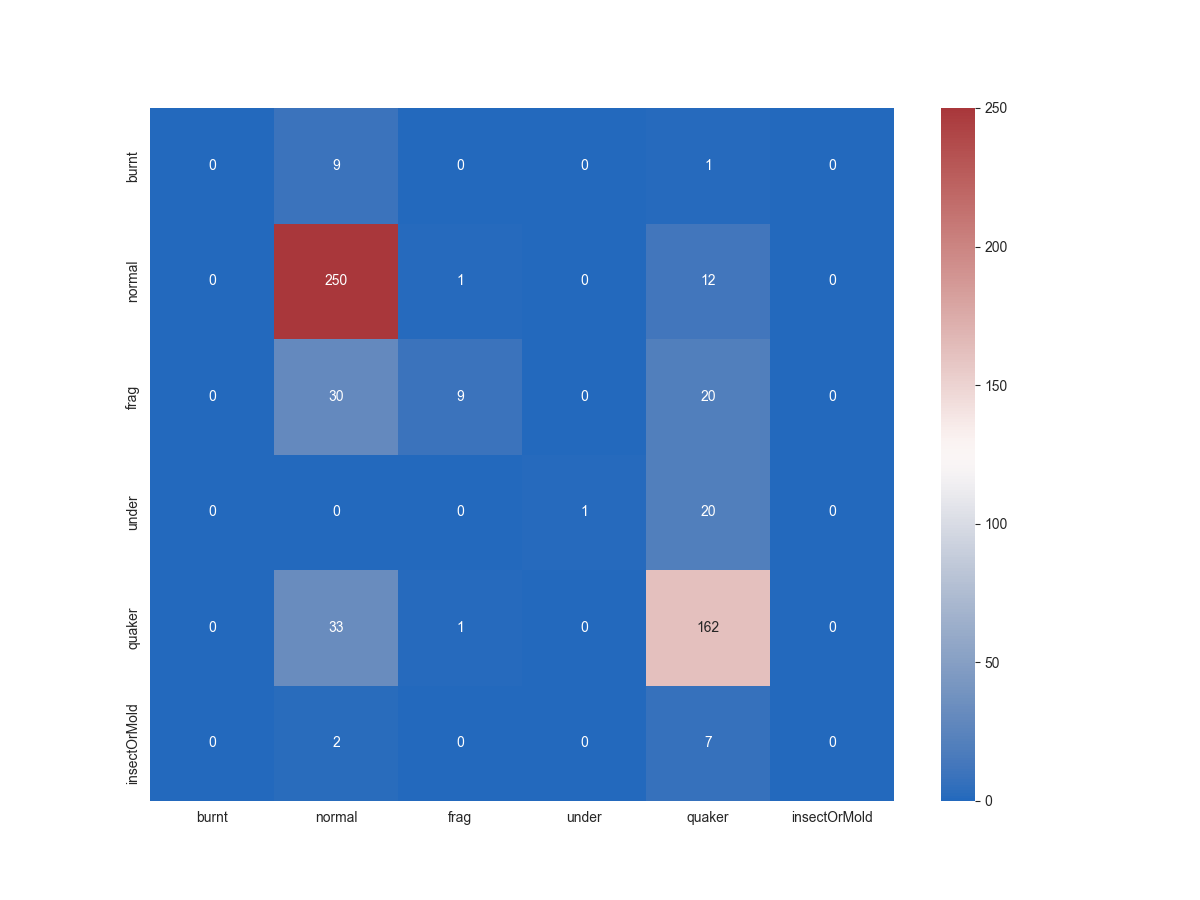
\includegraphics[width=\textwidth]{figures/confusionMatrices/KNN-28-neighbor-manhattan-histogram-32bins-noNorm-dimred}
    \caption{KNN-2}
    \label{fig:knn-2}
\end{wrapfigure}

\begin{figure}
    \centering
    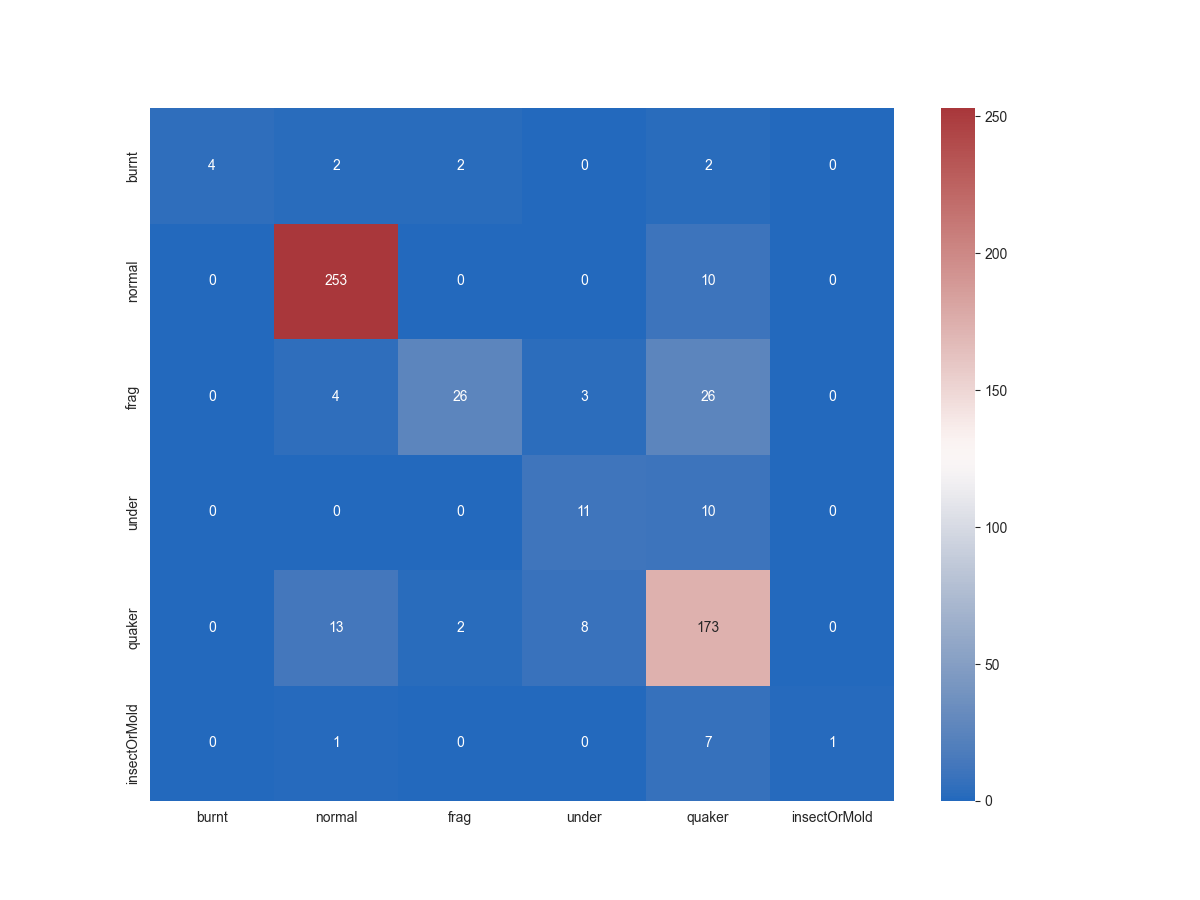
\includegraphics[width=\textwidth]{figures/confusionMatrices/mobileNet-no-pretraining0-5gamma}
    \caption{MobileNet (no pre-training)}
    \label{fig:mobileNetNoPt}
\end{figure}

\begin{figure}
    \centering
    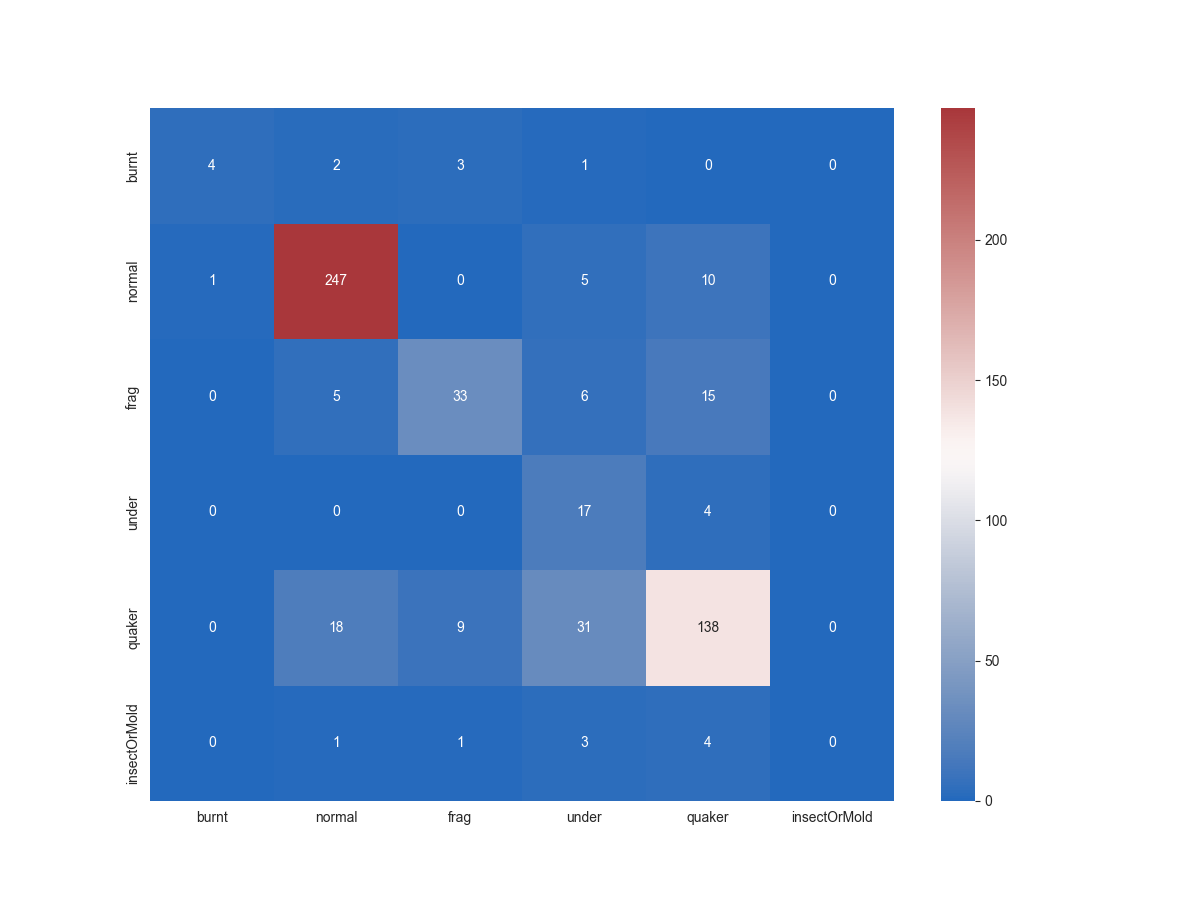
\includegraphics[width=\textwidth]{figures/confusionMatrices/shufflenet-no-pretraining0-5gamma}
    \caption{ShuffleNet (no pre-training)}
    \label{fig:shuffleNet}
\end{figure}

\begin{figure}
    \centering
    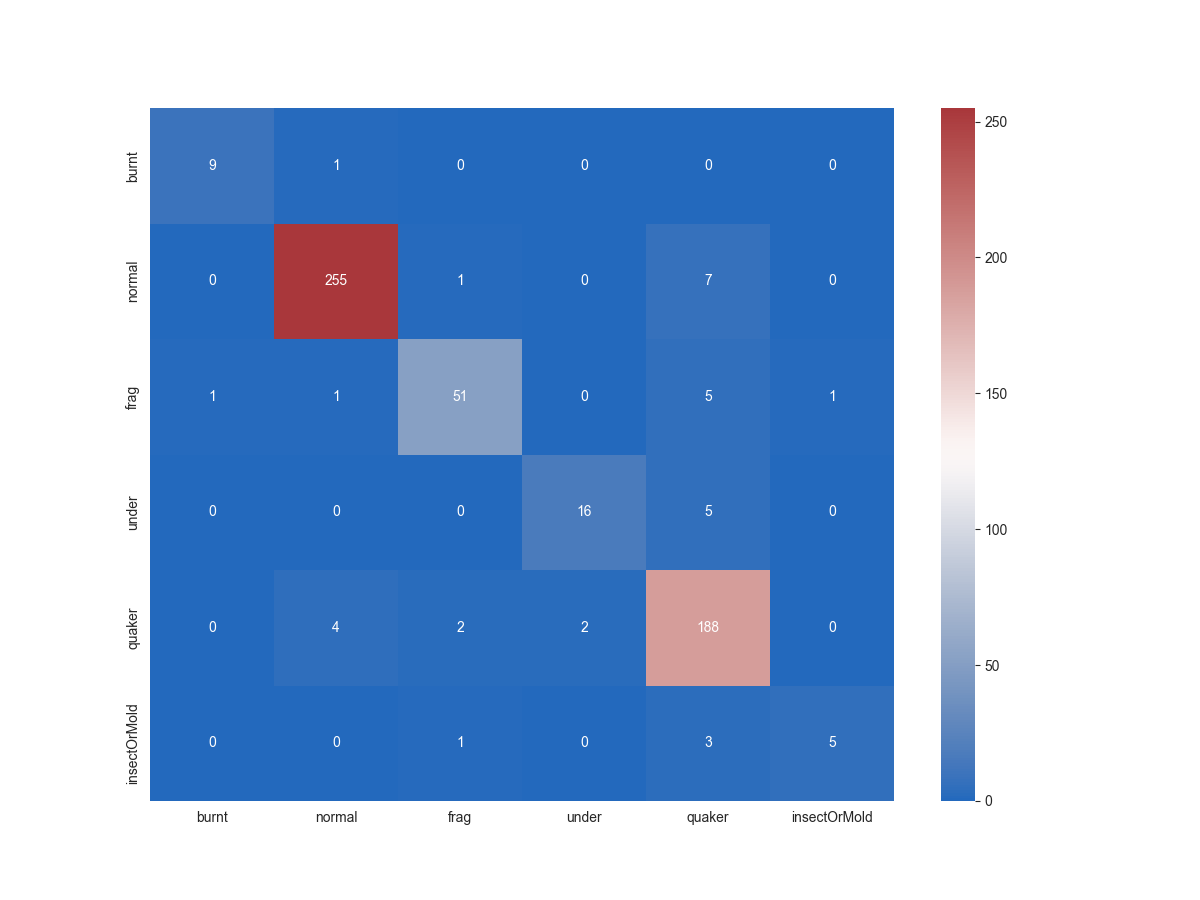
\includegraphics[width=\textwidth]{figures/confusionMatrices/resnet_18_93_acc}
    \caption{ResNet 18 (pre-trained)}
    \label{fig:resnet18}
\end{figure}

\begin{figure}
    \centering
    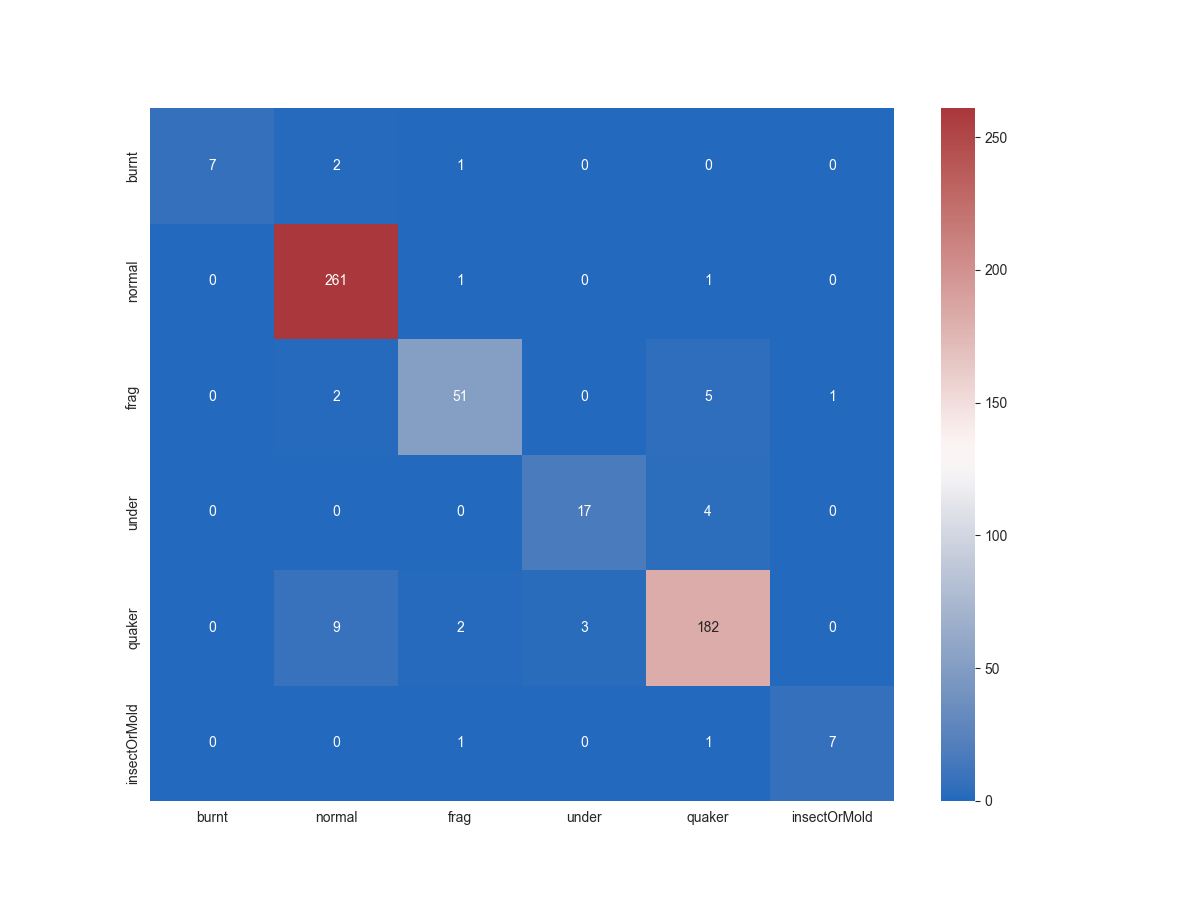
\includegraphics[width=\textwidth]{figures/confusionMatrices/resnet_34_whitebg_94_acc_8_batch}
    \caption{ResNet 34 (pre-trained)}
    \label{fig:resnet34}
\end{figure}

\begin{figure}
    \centering
    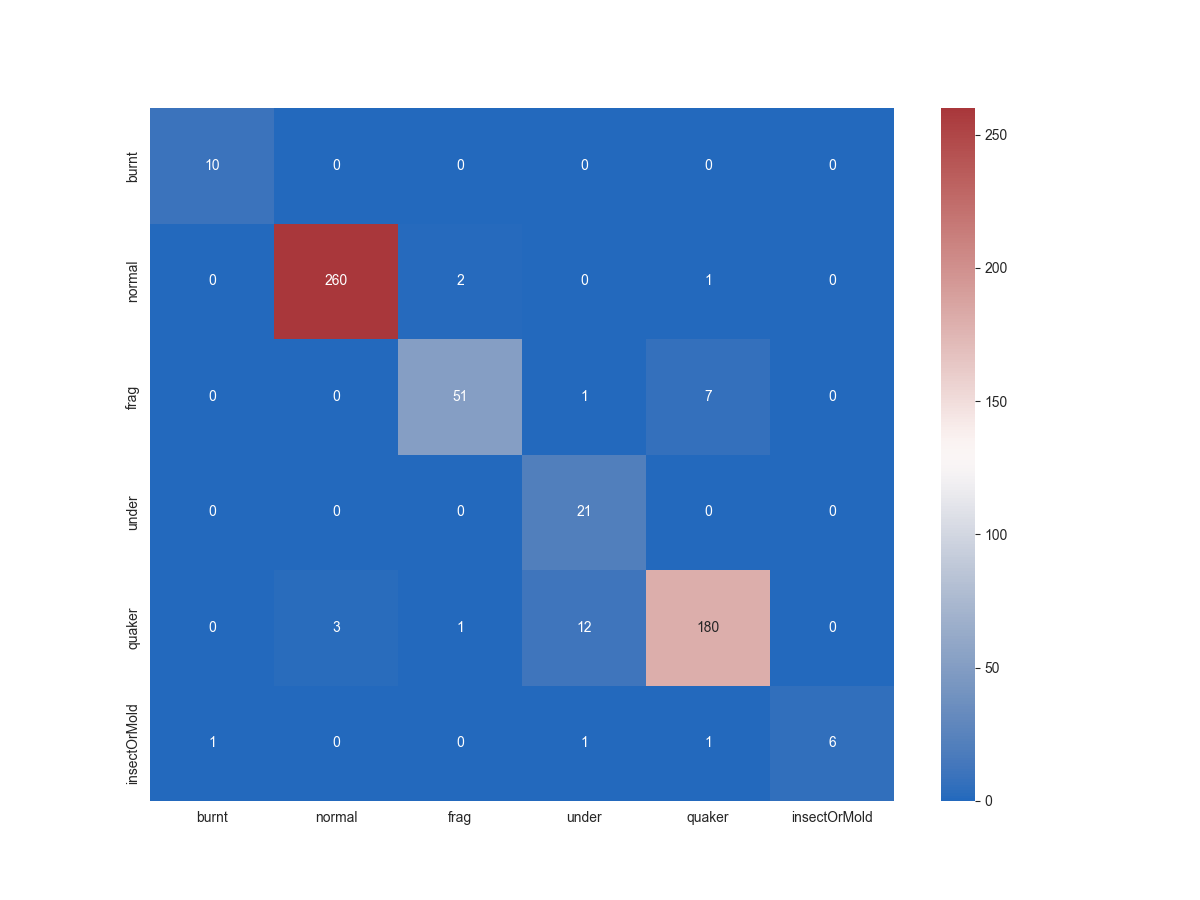
\includegraphics[width=\textwidth]{figures/confusionMatrices/resnet_50_95_acc}
    \caption{ResNet 50 (pre-trained)}
    \label{fig:resnet50}
\end{figure}

\begin{figure}
    \centering
    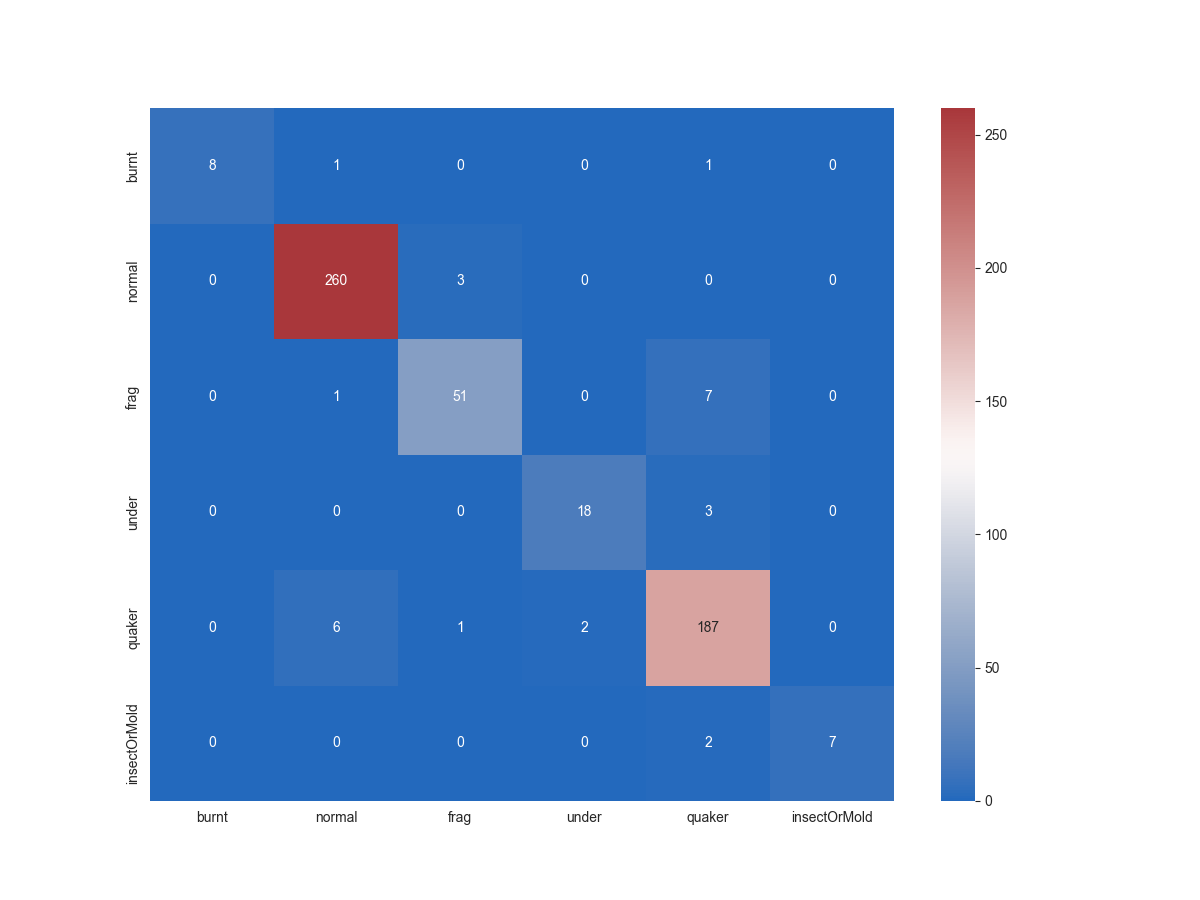
\includegraphics[width=\textwidth]{figures/confusionMatrices/mobilenet-95acc}
    \caption{MobileNet (pre-trained)}
    \label{fig:mobileNetPt}
\end{figure}

\begin{figure}
    \centering
    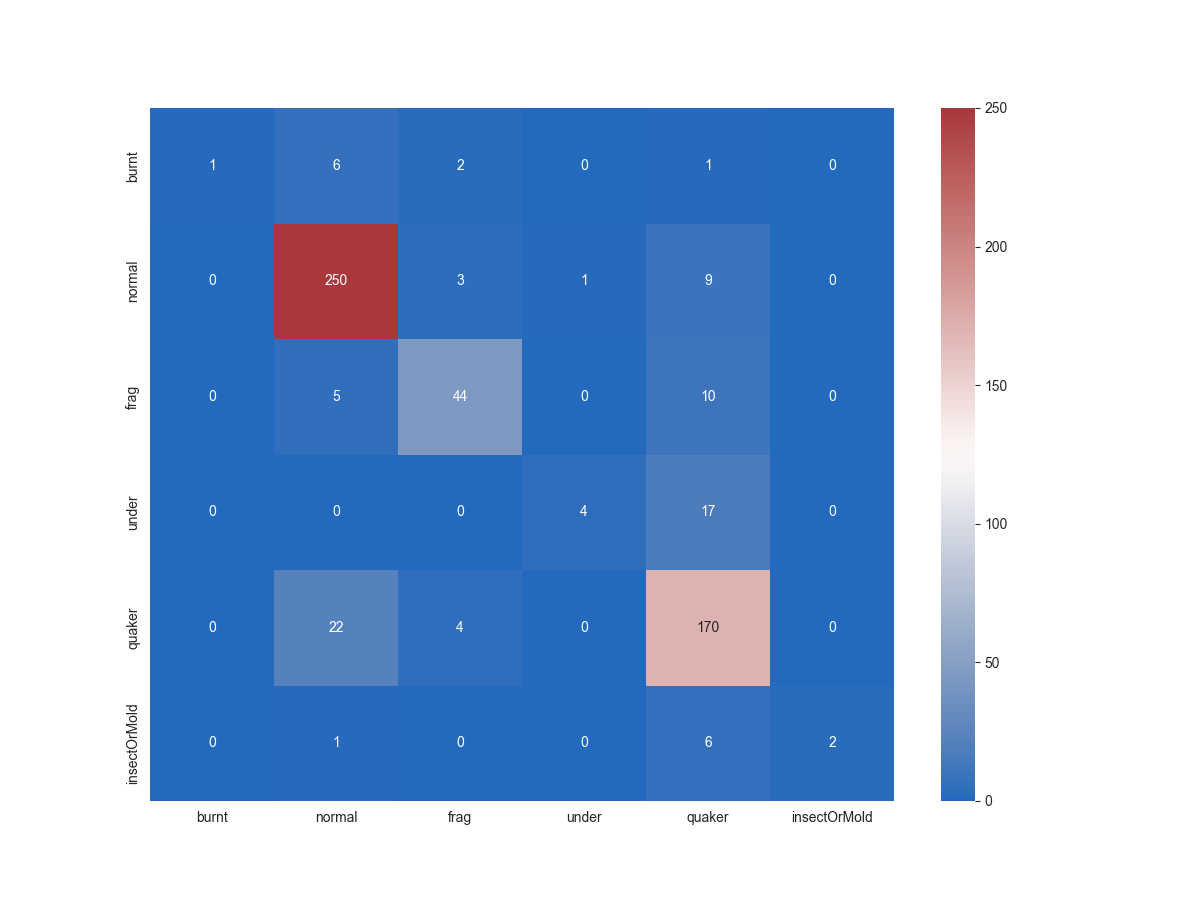
\includegraphics[width=\textwidth]{figures/confusionMatrices/swin_b_85_acc_4_batch}
    \caption{Swin transfomer (pre-trained, only last layer weights tracked)}
    \label{fig:swin}
\end{figure}


	\printbibliography
\end{document}